\documentclass[11pt,oneside]{book}
		\usepackage{listings}
		\usepackage{outlines}
		\usepackage{graphicx}
		\usepackage{tabulary}
		\usepackage{color}
		\usepackage[numbered]{bookmark}

		\title{The Computer Science Handbook}
		\author{Michael Young}

		\definecolor{dkgreen}{rgb}{0,0.6,0}
		\definecolor{gray}{rgb}{0.5,0.5,0.5}
		\definecolor{mauve}{rgb}{0.58,0,0.82}
		\lstset{
		  language=Java,
		  aboveskip=3mm,
		  belowskip=3mm,
		  showstringspaces=false,
		  columns=flexible,
		  basicstyle={\small\ttfamily},
		  numbers=none,
		  numberstyle=\tiny\color{gray},
		  keywordstyle=\color{blue},
		  commentstyle=\color{dkgreen},
		  stringstyle=\color{mauve},
		  breaklines=true,
		  breakatwhitespace=true,
		  tabsize=3
		}
		\graphicspath{ {../public_html/img/uploads/} }
		\makeatletter
		\def\maxwidth#1{\ifdim\Gin@nat@width>#1 #1\else\Gin@nat@width\fi}
		\begin{document}
		\maketitle
		\tableofcontents
		\chapter{ Getting Started }
    \section{ Getting Started }
    

The Computer Science handbook is a handbook designed to explain algorithms and data structures in a way that anyone can understand. Many websites (eg Wikipedia) contain lengthy and wordy explanations that are full of technical jargon. We have tried our hardest to simplify all language to make it easy to read without any math or computer science background. We hope to share our knowledge with you and we ask only one thing from you. You must learn something before you leave!

Before you get started with this handbook, it is highly recommended that you are already familiar with Java or C++ syntax. This handbook is not meaning for learning programming basics since there are other resources better suited for that task.

\subsection{Format}

Each article will have multiple sections to help you understand the content.

\subsubsection{Introduction}

The introduction section gives a brief overview of what the article is about. It will usually come with a prerequisite section which will contain topics that will be recommended to have been read before the article.

\subsubsection{Implementation}

The implementation section will be an implementation of the article in Java. It is recommended that you try to implement things yourself first before looking at the implementation. If you truly understand the concept, then you will never have to memorize a single line of code. The code will come from your understanding of how it works.

\subsubsection{Applications}

The applications section will be about real world applications of the concept that show why the concept is important.

\subsubsection{Exercises}

The exercises section contains practice problems to test if you truly understand the concept. Many of these questions come from real interview questions.

\part{ Fundamentals }
    \chapter{ Fundamentals }
        

Before we can learn about algorithms and data structures we must first learn how to analyze algorithms and data structures so we can apply them to the right needs.

It is highly recommended that you understand syntax for Java or C++ before you continue.


        \section{ Runtime and Memory }
        

Processing time and memory are two primary resources that computer programs use and it is important to analyze the limits we have. Computers are super fast at making calculations compared to humans, but humans have much more "memory" than computers currently do. For example, computers can add two 100-digit numbers together much more quickly than any human possibly can. However, the human brain can contain much more memory than humans.

Brains have trillions of connections between neurons and the estimated storage capacity is about 2.5 petabytes. That is approximately 340 years of TV shows that you could watch! Computers on the other hand, have much less memory than human brains. Standard computers have around 8GB of RAM and some higher end machines may have 16-32GB. Although hard-disks can store terabytes of memory, we use RAM (flash memory) when analyzing computer memory because it is much faster than disk storage. As an analogy, RAM can be thought of as grabbing an object in another room whereas disk memory is driving 20 min away to get that object.

The neurons and connections in our brains allow us to store an immense amount of information in our brains and allows us to easily recognize patterns much better than computers. For example it is very easy for us to identify different objects around us (e.g. we can easily differentiate between an apple and an orange), but it is difficult for a computer to do this for the countless number of objects in the world. However this is currently changing as more research is being done in "deep learning".

\vspace{10px}\begin{tabulary}{0.4\linewidth}{|l|l|l|l|l|l|l|l|l|l|l|l|l|l|l|l|l|l|l}\hline


   &
  Brain &
  Computer\\
\hline


  Memory &
  2.5 petabytes &
  16GB RAM\\

  Processing &
  60Hz &
  2.7GHz Quad Core\\

\hline\end{tabulary}

Note that a computer is 1,000,000,000 times faster than humans but humans can store 100,000 more information (approx. 340 years of TV shows).

\subsection{Limits}

There are many different methods of implementing different things but most of the time we care most about implementations that are the fastest and use the least amount of memory. Let's go through some basic benchmarks about computers that you should know. Adding two numbers takes a nanosecond (1 billionth of a second) for an average computer to process. For practical purposes, we'll assume that the average computer program can hold up to 1GB or RAM or about 250 million integers. We use RAM because it is flash memory and read/write is super fast in comparison to disk read/writes.

\vspace{10px}\begin{tabulary}{0.4\linewidth}{|l|l|l|l|l|l|l|l|l|l|l|l|l|l|l|l|l|l|l}\hline


  Memory &
  Operations (per seconds)\\
\hline


  1 GB (250,000,000 ints) &
  100,000,000 operations\\

\hline\end{tabulary}

\subsection{Big O Notation}

When we compare how efficient algorithms or data structures are to another, we want to be able to describe them such that they can be quantified. We use something called Big O notation to do this. Many algorithms and data structures will have its time and space complexities depend on the size of the inputs. The Big O notation takes the largest factor of an input to compare computation times / memory usage. When we take the largest factor, we ignore smaller factors, coefficients and constants because they do not matter at very large values. For example: O(3n$^{2}$ + 12n + 20) is simply O(n$^{2}$) because it is the largest factor.

Here is a list of common Big O notations based on complexity:

\vspace{10px}\begin{tabulary}{0.4\linewidth}{|l|l|l|l|l|l|l|l|l|l|l|l|l|l|l|l|l|l|l}\hline


  Big O &
  Limit of N for 1 second (Standard processor)\\
\hline


  O(1) Constant Time &
  runtime independent of N\\

  O(log N) Sublinear time &
  a very big number\\

  O(N) Linear Time &
  100,000,000\\

  O(N log N) &
  5,000,000\\

  O(N$^{2}$) Quadractic Time &
  10000\\

  O(N$^{3}$) Cubic Time &
  450\\

  O(2$^{N}$) Exponential Time &
  27\\

  O(N!) Factorial Time &
  11\\

\hline\end{tabulary}

Keep in mind that in a couple of years as technology improves, this chart will be outdated.

\subsection{Runtime Analysis}

Let us examine a function that takes in an array of size N and returns the maximum element. In a program we are usually concerned with two complexities: memory and time.

Code:

\begin{lstlisting}
int findMax(int[] array){
  int maxVal = array[0]; //O(1) memory to store max element, O(1) time for assignment
  for(int i=1;i<array.length;i++){ //O(n) loop runtime
      if(maxVal < array[i]){ //O(1) to compare runtime
         maxVal = array[i]; //O(1) to assign new value runtime
     }
  }
}
\end{lstlisting}

Memory: The array takes O(N) memory and storing the max value is O(1) more memory. but usually when analyzing programs, we ignore the input memory sizes and take into account additional memory that is required to produce the output. So the memory footprint of the function is O(1).

Time: The first assignment of maxVal takes O(1). The loop runs N-1 times and of each of those N-1 times it checks if the current array element is greater than the current max which takes O(1). If it is greater, then we reassign maxVal which is O(1). When analyzing time complexity, we usually take worst case so we have: O(1+(N-1)(2)) and this simplifies to O(N) since it is the largest factor.

\subsubsection{Example}

Suppose we have a function that zeroes a 2D NxN array.

\begin{lstlisting}
void zeroArrays(int[][] grid){
  //O(n) loop
  for(int i=0; i<grid.length;i++){
    //O(n) loop
    for(int j=0;j<grid[i].length;j++){
      //O(1)
      grid[i][j] = 0;
    }
  }
}
\end{lstlisting}

There are NxN cells we need to set to 0 so we need O(N$^{2}$) operations. We can also think of it as another way. There are two nested loop and each loop is O(n) so we multiply them and O(n) x O(n) = O(n$^{2}$). Generally, when we have nested loops, we multiple their complexities.

\subsubsection{Example}

Suppose we have another function that prints out the binary backwards for each number from 1 to N.

\begin{lstlisting}
void binaryNumbers(int n){
    for(int x = 1; x < n; x++){
        int bin = x;
        while(bin > 0){
            System.out.print(bin % 2);
            bin = bin / 2;
        }
        System.out.println();
    }
}
\end{lstlisting}

For each number x, it will take O(log x) to convert the number to binary and we do this N times so the runtime is: O(n log n).

\part{ Recursion }
    \chapter{ Recursion }
        \section{ Recursion }
        

Next: Advanced Recursion

Recursion is process that repeats itself in a similar way. Anything that has its definition nested inside itself is considered to be recursive. For example GNU stands for GNU not Unix!. Expanding this acronym gives us ((GNU not Unix) not Unix!). As you can see this will go on forever and GNU's definition is nested inside itself so it is recursive. The Fibonacci sequence is also recursive: F(n) = F(n-1)+F(n-2). Inside the function F, we see two more F's!

In computer science infinite looping is not good because computers do not know how to terminate so we need some way to terminate it. We will call a stopping point the base case. A base case is the case where the function will stop and everything should eventually reduce to a base case. For the Fibonacci sequence, the base case is F(0) = 1 and F(1) = 1 and we can see that for all N$>$1, the Fibonacci sequence will reach the base case.

So for something to be recursive in computer science, it needs:

\begin{itemize}
\item a recursive definition (contained in itself) and 
\item a base case that all valid inputs will eventually reach
\end{itemize}

Template for recursion:

\begin{lstlisting}
recursion(parameter)
    if base_case (parameter):
        stop
    recursion( operation(parameter) )
\end{lstlisting}

\begin{itemize}
\item recursion is the recursive function
\item base\_case is the check if the parameter has reached the base case
\item operation reduces the parameters towards the base case
\end{itemize}

\subsection{Factorial}

Let's look at a simple recursive function: factorial.

1! = 1

n! = 1 * 2 * 3 .... n.

Or we could write it as n! = (n-1)! * n. We now see that in this form, the factorial function is defined within itself which makes it recursive. Our base case is 1! = 1.

Example:

4!

= 3! * 4

= 2! * 3 * 4

= 1! * 2 * 3 * 4

= 1 * 2 * 3 * 4

= 24

\subsubsection{Formalization}

\begin{lstlisting}
Let f(n) be the nth factorial number where n is a positive integer.

Base case:
f(1) = 1

Recurrence:
f(n) = f(n-1) * n

Example:
f(4) 
= f(3) * 4
= f(2) * 3 * 4
= f(1) * 2 * 3 * 4  [Base Case]
= 1 * 2 * 3 * 4
= 24
\end{lstlisting}

\subsubsection{Implementation}

\begin{lstlisting}
int factorial(int n){
   if(n == 1)return 1;
   return factorial(n - 1) * n;
}
\end{lstlisting}

\subsection{Sum of digits of a string}

We can use recursion in many places and we can apply it to simple problems that you probably have not thought about. Summing the digits of a string can be done using simple loop but we can also use recursion to do it.

Let's say we have the string '23528'. The total is equal to the first digit + the sum of the rest of the digits. 2 + '3528'. We can do the exact same thing for the rest of the digits: the second digit + the sum of the rest of the digits and keep doing this until we have no more digits.

\begin{itemize}
\item f('23528')
\item f('3528') + 2
\item f('528') + 3 + 2
\item f('28') + 5 + 3 + 2
\item f('8') + 2 + 5 + 3 + 2
\item f('') + 8 + 2 + 5 + 3 + 2
\item 0 + 8 + 2 + 5 + 3 + 2
\item 20
\end{itemize}

\subsubsection{Formalization}

\begin{lstlisting}
Let sum(string) be the sum of digits in a string
Let n be the length of the string

For simplicity, let string[x..y] be the substring of the string from index x to index y. 
The starting index will be 1.

Example: 
string = 'abcd'.
string[1..3] = 'abc'
string[1..1] = ''
string[1] = 'a'

Base case:
sum(empty) = 0

Recurrence:
sum(string) = sum(string[2..n]) + int(string[1])

Example:
sum('23528')
= sum('3528') + 2
= (sum('528') + 3) + 2
= ((sum('28') + 5) + 3) + 2
= (((sum('8') + 2) + 5) + 3) + 2
= ((((sum('') + 8) + 2) + 5) + 3) + 2
= ((((0 + 8) + 2) + 5) + 3) + 2
= 20
\end{lstlisting}

\subsubsection{Implementation}

\begin{lstlisting}
int sum(string str){
   int n = str.length();
   if(n == 0){
       return 0;
    }
   else{
     int charToNum = (str.charAt(0) - '0');
     return sum(str.substring(1, n)) + charToNum;
   }
}

sum('23528');
\end{lstlisting}

\subsection{Count}

Let's say we have an string of N characters and we want to find the number of times the letter 'c' appears. This time we need to add some logic to the problem.

If the first letter of the string is a 'c', then we can add 1 to the count. Otherwise, we don't add anything. We can do the exact same thing for the substring without the first letter. If the second letter of the string is a 'c', we add 1 other we don't add anything etc.

For example we have the string 'cacaec'. Since the first letter is a 'c' we add 1 to the count. Then we remove the first letter and get 'acaec', the first letter is not a 'c' so we don't add to the count. We keep reducing this way until we get an empty string and we return the count.

\begin{itemize}
\item 'cacaec'
\item 'acaec' +1
\item 'caec' + 0 + 1
\item 'aec' + 1 + 0 + 1
\item 'ec' + 0 + 1 + 0 + 1
\item 'c'  + 0 + 0 + 1 + 0 +1
\item '' + 1 + 0 + 0 + 1 + 0 + 1
\item 0 + 1 + 0 + 0 + 1 + 0 + 1
\item 3
\end{itemize}

\subsubsection{Formalization}

\begin{lstlisting}
Let count(string) be the number of 'c's in the string

For simplicity, let string[x..y] be the substring of the string from x to y.
Example: 
string = 'abcd'.
string[1..3] = 'bcd'

Base case:
count(empty) = 0

Recurrence:
count(string) =  {if string[n]=='c'  count(string[2..n])+1
                 {else               count(string[2..n])

Example:
count('cacaec')
= count('acaec') + 1
= (count('caec') + 0) + 1
= ((count('aec')+ 1) + 0) + 1
= (((count('ec') + 0) + 1) + 0) +1
= ((((count('c') + 0) + 0) + 1) + 0)+1
= ((((count('') + 1) + 0) + 0) + 1) + 0) + 1
= ((((0 + 1) + 0) + 0) + 1) + 0) + 1
= 3
\end{lstlisting}

\subsubsection{Implementation}

\begin{lstlisting}
int count3(string str){
   int n = str.length();
   if(n == 0)return 0;
   if(str.charAt(0) == 'c'){
      return count3(str.substring(1, n)) + 1;
   }
   else{
     return count3(str.substring(1, n));
   }
}

count3('cacaec');

\end{lstlisting}

\subsection{Calculate Exponential}

Let's say we wanted to find x$^{n}$ and for the sake of this problem we want the last four digits of that number. Note that 267$^{4}$ mod 10000 = (267$^{3}$ mod 10000) * 267 mod 10000. This is important because it means we can take the last 4 digits in each step instead of having to compute the giant exponent and then taking the last 4 digits. We can do this problem very easily by using a simple loop, but we can do better by using recursion. By definition of exponents, x$^{a}$ * x$^{a}$ = x$^{2a}$. Using this we can see that if n is divisible by 2, then x$^{n}$ = x$^{n/2}$ * x$^{n/2}$.

For example 5$^{4}$ = 5$^{2}$ * 5$^{2}$

But let's take a look at x$^{n/2}$. If n is even we can do the exact same thing! x$^{n/2}$ = x$^{n/4}$ * x$^{n/4}$. We are solving a reduced version of the same problem so we have a recurrence relation. The base case is simple: x$^{1}$ = x.

But what if n is odd and not 1? Then we have x$^{n}$ = x$^{n/2}$ * x$^{n/2}$ * x. Thus our recursive function has 3 different cases: the base case, even case and odd case.

\subsubsection{Formalization}

\begin{lstlisting}
Let exp(b,n) be b^n

Base case:
exp(b,1) = 1  [Since b^1 = b]

Recurrence:
exp(b,n) = {if n divisible by 2    exp(b,n/2)^2 % 10000
           {else                   (exp(b,n/2)^2)*b % 10000

Example: (for simplicity, leave out the modulus)
exp(3,10)
= exp(3, 5) ^ 2
= (exp(3, 2) ^ 2)) * 3) ^ 2
= (((exp(3, 1) ^ 2) * 3) ^ 2) [Base case]
= (((3 ^ 2) ^ 2) * 3) ^ 2)
= ((9 ^ 2) * 3) ^ 2)
= (81 * 3) ^ 2
= (243) ^ 2
= 59049
\end{lstlisting}

\subsubsection{Implementation}

\begin{lstlisting}
int exponent(int b, int n){
   if(n == 1)return b;
   if(n % 2 == 0){
     int x = exponent(b, n / 2);
     return (x * x) % 10000;
   }
   else{
     int x = exponent(b, n / 2);
     return (x * x * b) % 10000;
   }
}

\end{lstlisting}

\subsection{Exercises}

\begin{enumerate}
\item Given an array of N integers, write a recursive function to get the sum
\item Given a string S, write a recursive function to determine if it is a palindrome.
\item Given a number N, write a recursive function to output the number in binary.
\item Given a string S, write a recursive function to return a reversed string
\end{enumerate}

        \section{ Advanced Recursion }
        

Prerequisites: Recursion

Next: Intermediate Recursion, Backtracking, Dynamic Programming

Recursion can sometimes be very difficult to wrap your head around because when you try to go deeper, it only keeps getting deeper. It is sometimes hard to figure out the recurrence relation, but once you do, the problem becomes simple to solve.

\subsection{Number of paths}

Suppose we have a grid of N rows and M columns. How many ways are there to get from the bottom left corner to the top right corner using the intersection points and only going upwards or rightwards?

\vspace{5px}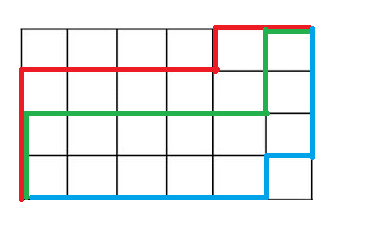
\includegraphics[width=\maxwidth{\textwidth}]{recursion_grid.png}

We see that the only way to reach an intersection is to come from the left or from the bottom. So the number of ways to reach an intersection is the number of ways to reach the intersection to the left plus the number of ways to reach the intersection on the bottom.

So more accurately, the number of ways to get to intersection N x M is the sum of the ways to get to the intersection N-1 x M and the intersection N x M-1. However, the number of ways to reach the intersection N-1 x M is the sum of the number of ways to the intersection N-2 x M and N-1 x M-1. As we can see, we are solving a reduced version of the same problem. Thus we have a recurrence relation.

The base case is any intersection on the left side or bottom side. There is only one way to reach the intersections by either going only up or only going right.

\subsubsection{Formalization}

\begin{lstlisting}
Let path(x,y) be the number of ways to get to the intersection at x and y

Base case:
paths(1,y) = 1
paths(x,1) = 1

Recurrence:
paths(x,y) = paths(x-1,y) + paths(x,y-1)

Example:
paths(3,5)
= paths(2,5) + paths(3,4)
= paths(1,5) + paths(2,4) + paths(2,4) + paths(3,3)
= 1 + paths(1,4) + paths(2,3) + paths(1,4) + paths(2,3) + paths(2,3) + paths(3,2)
= 1 + 1 + paths(1,3) + paths(2,2) + 1 + paths(1,3) + paths(2,2) + paths(1,3) + paths(2,2) + paths(2,2) + paths(3,1)
= 1 + 1 + 1 + paths(1,2) + paths(2,1) + 1 + 1 + path(1,2) + paths(2,1) + 1 + paths(1,2) + paths(2,1) + ....
= 15
\end{lstlisting}

Example of what the grid should look like

\vspace{5px}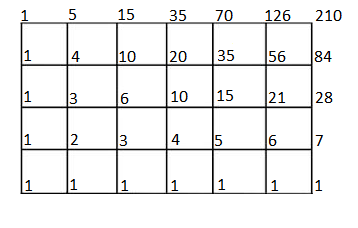
\includegraphics[width=\maxwidth{\textwidth}]{recursion_grid2.png}

\subsubsection{Implementation}

\begin{lstlisting}
int paths(int n,int m){
   if(n == 1 || m == 1){
        return 1;
   }
   return paths(n - 1, m) + paths(n, m - 1);
}
\end{lstlisting}

\subsection{Towers of Hanoi}

There are three poles and N disks where each disk is heaver than the next disk. In the initial configuration, the discs are stacked upon another on the first pole where the lighter discs are above the heavier discs. We want to move all the discs to the last pole with the following conditions:

\begin{itemize}
\item Only one disc can be moved from one pole to another at a time.
\item The discs have to be stacked such that all the lighter discs are on top of the heavier ones.
\end{itemize}

Lets' try to make this problem simpler. To move N discs from the first pole the the last pole we need to move N-1 discs to the middle pole, then move the Nth disc to the last pole, and then move all N-1 discs from the middle pole back on to the last pole.

Let the starting pole be the first pole, the helper pole be the middle pole and the destination pole the third pole.

\vspace{5px}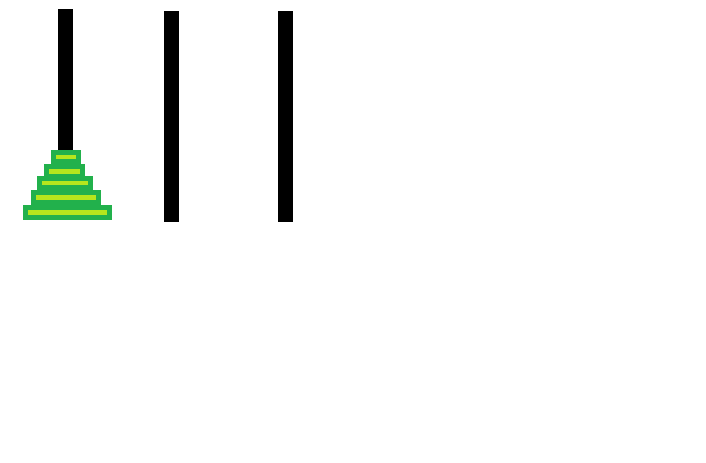
\includegraphics[width=\maxwidth{\textwidth}]{hanoi.png}

To move N discs from the starting pole to the destination pole:

Step 1:

We need to move N-1 discs from the starting pole to the helper pole.
\vspace{5px}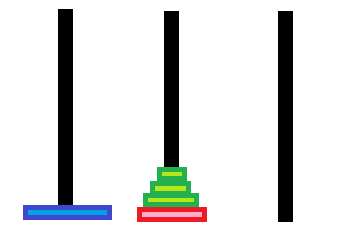
\includegraphics[width=\maxwidth{\textwidth}]{hanoi2.png}

Step 2:

We need to move the Nth disc from the starting pole to the destination pole.
\vspace{5px}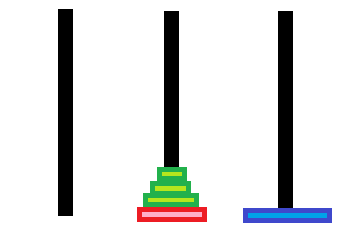
\includegraphics[width=\maxwidth{\textwidth}]{hanoi3.png}

Step 3:

We need to move N-1 discs from the helper pole to the destination pole.
\vspace{5px}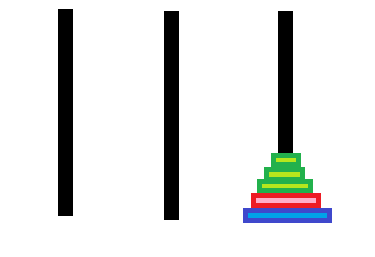
\includegraphics[width=\maxwidth{\textwidth}]{hanoi4.png}

We can see that Step 2 is easy, all we have to do is move that one disc. But for Step 1 and Step 3, we have to move N-1 discs. How can we move N-1 discs to the middle pole?

We see that we can use the same reasoning: we need to move N-2 discs to the third pole. Then we need to move the N-1 disc to the second pole and then move N-2 discs from the third pole to the second pole. Note that the Nth disc does not matter at all in this case since we can move any disc on top of it and we can pretend as if it doesn't exist.

In this case, the starting pole is the first pole, the helper pole is the third pole and the destination pole is the middle pole.

\vspace{5px}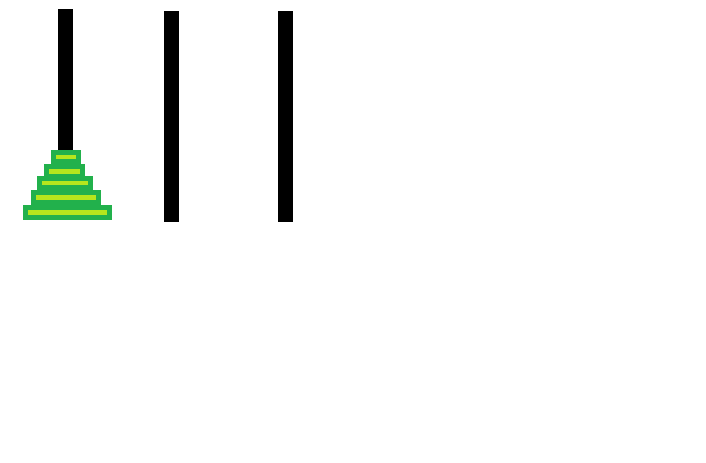
\includegraphics[width=\maxwidth{\textwidth}]{hanoi.png}

To move N-1 discs from starting pole to destination pole:

Step 1:

We need to move N-2 discs from starting pole to helper pole

\vspace{5px}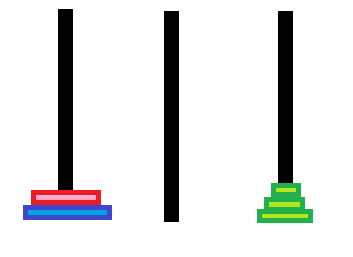
\includegraphics[width=\maxwidth{\textwidth}]{hanoi5.png}

Step 2:

We move the N-1th disc from the starting pole to the destination pole

\vspace{5px}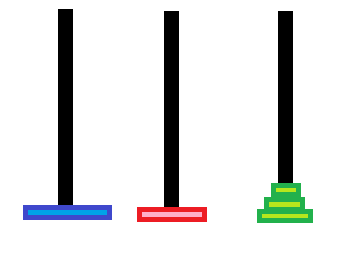
\includegraphics[width=\maxwidth{\textwidth}]{hanoi6.png}

Step 3:

We move N-2 discs from the helper pole to the destination pole.

\vspace{5px}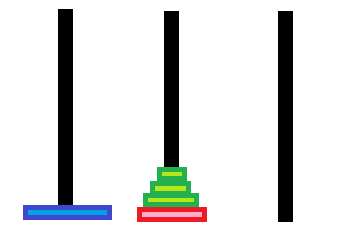
\includegraphics[width=\maxwidth{\textwidth}]{hanoi2.png}

As we can see, the steps to move N discs are the exact same as to move N-1 discs! The only difference is that the actual poles are different but we the steps are the same relative to their roles (starting, helper and destination). We are solving a reduced version of the same problem and so have a recurrence.

In Step 1, when we move N-1 discs from start to helper, the new helper is the old destination and the new destination is the old helper.

In Step 3, when we move N-1 discs from the helper to the destination, the new helper is the start pole, and the new start pole is the helper

\subsubsection{Formalization}

\begin{lstlisting}
Let f(N,start,helper,dest) be the steps to move N discs from the start to dest

Base case:
f(1,start,helper,dest) = Move from (start) to (dest)

Recurrence:
f(N,start,helper,dest)

=

f(N - 1, start, dest, helper)
Move from start to dest
f(N - 1, helper, start, dest)

Example:
Let A, B, C be pole 1, 2, 3

f(4,A,B,C) 

=

f(3,A,C,B)
Move from A to C
f(3,B,A,C)

=

f(2,A,B,C)
Move from A to B
f(2,C,A,B)
Move from A to C
f(2,B,A,C)
Move from B to C
f(2,A,B,C)

=

f(1,A,C,B)
Move from A to C
f(1,B,A,C)
Move from A to B
f(1,C,B,A)
Move from C to B
f(1,A,C,B)
Move from A to C
f(1,B,C,A)
Move from B to C
f(1,A,B,C)
Move from B to C
f(1,A,C,B)
Move from A to C
f(1,B,A,C)

=

Move from A to B
Move from A to C
Move from B to C
Move from A to B
Move from C to A
Move from C to B
Move from A to B
Move from A to C
Move from B to A
Move from B to C
Move from A to C
Move from B to C
Move from A to B
Move from A to C
Move from B to C

\end{lstlisting}

\subsubsection{Implementation}

\begin{lstlisting}
void hanoi(int N, int start, int helper, int destination){
    if(N == 1){
        System.out.println("Move " + start + " to " + destination);
    }else{

        //Move N-1 disks from start to helper
        hanoi(N-1, start, destination, helper);

        //Move 1 disk from start to end
        hanoi(1, start, helper, destination);

        //Move N-1 disks from helper to end
        hanoi(N - 1, helper, start, destination);
    }
}
hanoi(4, 1, 2, 3);
\end{lstlisting}

\subsection{Permutations}

A permutation is an arrangement of the original set of elements.

For example permutations of A,B,C,D,E,F:

\begin{itemize}
\item D,E,F,C,B,A
\item F,C,D,B,A,E
\item B,D,A,E,F,C
\item A,B,C,D,E,F
\end{itemize}

Given a string S of length N, how can we generate all permutations?

Let's assume that we have a list of permutations for the substring of S of N-1 characters. Then to get the permutations for the string of length N, all we need to do is insert the Nth character in between all the positions of each permutation of N-1 characters. For example permutation of A,B,C,D.

We can manually find the permutations of A,B,C.

\begin{itemize}
\item A,B,C
\item A,C,B
\item B,A,C
\item B,C,A
\item C,A,B
\item C,B,A
\end{itemize}

If we insert the letter D between each letter for every permutation in N-1 letters, we get:

\begin{itemize}
\item D,A,B,C
\item A,D,B,C
\item A,B,D,C
\item A,B,C,D
\item D,A,C,B
\item A,D,C,B
\item A,C,D,B
\item A,C,B,D
.... etc
\end{itemize}

And we can guarantee that every new permutation will be unique. (Try to prove that to yourself).

But let's look at how we can get the permutation of A,B,C. We can also get all the permutations of the string by taking the permutations of A,B and inserting C in all the positions for all substrings.

Substrings of A,B

\begin{itemize}
\item A, B
\item B, A
\end{itemize}

Insert C for all positions for all permutations

\begin{itemize}
\item C,A,B
\item A,C,B
\item A,B,C
\item C,B,A
\item B,C,A
\item C,B,A
\end{itemize}

We see that we are solving the same reduced problem thus we have a recurrence relation. To get the permutations of a string N, we take the string[1..N-1] and we insert the Nth character at every position for each permutation of the N-1 substring. The base case of an empty string is simply an empty string. Permutation of an empty string is an empty list.

For simplicity, S[i..j] will mean the substring from including i to excluding j.

\begin{lstlisting}
Let P(S) be the list of permutations for the string S of length N

Base case:
P('') = []

Recurrence:
Let N = length of string S
P(S) = ps[0..i] + S[N] + ps[i..N] for i in 0..N, for ps in P(S[0..N-1])

Example:
P('ABC')
=

\end{lstlisting}

\subsubsection{Implementation}

\begin{lstlisting}
Vector<String> permutation(String s){
   int n = s.length;
   Vector<String> vec = new Vector<String>();
   if(s.length==0)return vec;
   Vector<String> subvec = permutation(s.substring(0,n-1));
   for(int i=0;i<subvec.size();i++){
      String ps = subvec.get(i);
      for(int j=0;j<n;j++){
         vec.push(ps.substring(0,j)+s.charAt(n)+ps.substring(j,n-1));
      }
   }
   return vec;
}
\end{lstlisting}

\subsection{Exercises}

\begin{enumerate}
\item Given a string S, write a recursive function to generate all substrings
\item Write a solution for hanoi towers but with the restriction that discs can only be moved from adjacent poles. (You can move a disc from A to B but not A to C because they are not adjacent)
\end{enumerate}

\part{ Data Structures }
    

Data structures are different ways of storing data such that they optimize certain data operations such as retrieval and insertion. Although many of these data structures are already built into various languages, it is important to understand how they work. By understanding the implementations, we can have a sense of which data structure to use for different scenarios.

An abstract data type is a conceptual model for representing data. An abstract data type tells what it should do as opposed to how it should work. It will tell us what operations it should have but should not tell us how to implement them.

For example, a bottle should be able to hold water and allow us to drink from. This tells us what it should do but we don't need to know how it works or how it is made. A plastic water bottle is an implementation of a bottle. It holds water in its interior and allows us to drink by unscrewing the cap and letting us pour water down our throat. A thermos is also an implementation of the bottle, it holds fluid inside it, but this thermos has a lid that can be popped open and water can come from it. A thermos and plastic water bottle are different implementations as they are made differently and used differently, but they fundamentally do what a bottle is supposed to do: store liquid, and provide a way to drink. A bottle does not actually exist, but types of bottles do.

\vspace{5px}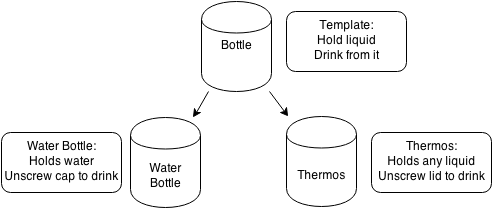
\includegraphics[width=\maxwidth{\textwidth}]{bottle.png}

Some implementations of abstract data types are better than others for different purposes. For example plastic water bottles are very cheap whereas a thermos is more expensive but a thermos can hold hot water and keep it warm for a long period of time. When selecting a data structure, we should analyze the efficiencies of data operations that we will do most often.

\vspace{5px}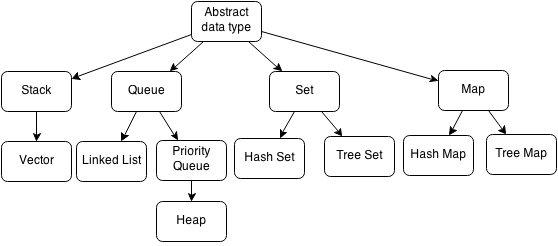
\includegraphics[width=\maxwidth{\textwidth}]{adt.png}

For more intermediate data structures, read the advanced data structures page.


    \chapter{ Stack }
        \section{ Stack }
        

Imagine a stack of plates at a buffet, the plates are taken from the top and are also replaced from the top. The first plate to go in will be the last plate to come out. The last plate to go in will be the first to come out. This structure is called a stack.

A stack is an abstract data type with the property that it can remove and insert elements following a FILO (First In Last Out) structure. The first element to be inserted must be the last element to be removed and the last element to be inserted must be the first element to be removed. Sometimes, removal is called "pop" and insertion is called "push".

Example of push:

\vspace{5px}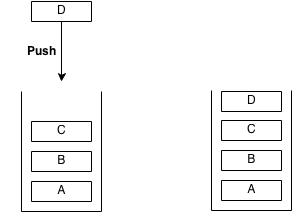
\includegraphics[width=\maxwidth{\textwidth}]{stack.png}

Example of pop:

\vspace{5px}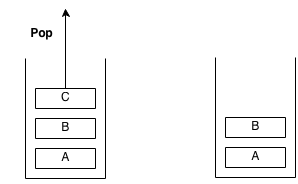
\includegraphics[width=\maxwidth{\textwidth}]{stack2.png}

Stacks are used for function calls on the memory stack. Whenever a function is called, it is placed on the memory stack with its variables and when it is returning a value, it is popped off the stack.

A stack is usually implemented as a vector.

\subsection{Implementation}

\vspace{10px}\begin{tabulary}{0.4\linewidth}{|l|l|l|l|l|l|l|l|l|l|l|l|l|l|l|l|l|l|l}\hline


  Implementation &
  Pop &
  Push\\
\hline


  Vector &
  O(1) &
  O(1)\\

\hline\end{tabulary}

\subsection{Exercises}

\begin{enumerate}
\item Given a string of brackets of either () or [], determine if the bracket syntax is legal (every opening bracket has a closing bracket from left to right).

Legal syntax:

\begin{itemize}
\item ( [ ( ) [ ] ] )
\item ( ) ( ) [ ] ( ) ( )
\end{itemize}

Illegal syntax:

\begin{itemize}
\item ( ( ) ]
\item ( ) [ ( ] )
\end{itemize}
\end{enumerate}

        \section{ Vector }
        

Prerequisites: Arrays, Stack

Source on Github

A vector is a stack that is implemented as an array. It is very similar to an array, but it is more flexible in terms of size. Elements are added and removed only from the end of the array. When more elements are added to the vector and the vector is at full capacity, the vector resizes itself and reallocates for 2*N space. When using an vector we can keep adding elements and let the data structure handle all the memory allocation.

\vspace{10px}\begin{tabulary}{0.4\linewidth}{|l|l|l|l|l|l|l|l|l|l|l|l|l|l|l|l|l|l|l}\hline


  Operation &
  Get &
  Push &
  Pop &
  Insert &
  Delete\\
\hline


  Time Complexity &
  O(1) &
  O(1) &
  O(1) &
  O(n) &
  O(n)\\

\hline\end{tabulary}

\subsection{Class}

There is a builtin Vector class already, but we will go through the implementation of a simple integer vector class to understand how the data structure works.

In our vector class, we need to store the element and the size of the current vector.

\begin{lstlisting}
class Vec{
    private int[] arr; //Storage of elements
    private int size; //Current size
}

//Constructor
publc Vec(int startSize){
    arr = new int[startSize];
    this.size = 0;
}

\end{lstlisting}

\subsection{Resize}

Resize will be used to resize the current size of elements. We create a new array of two times the size of the old one and copy the old array over.

\vspace{5px}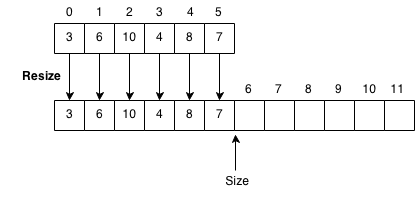
\includegraphics[width=\maxwidth{\textwidth}]{vector3.png}

\begin{lstlisting}
public void resize(){
    int[] newArr = new int[2*arr.length];
    for(int i=0;i<end;i++){
        newArr[i] = arr[i];
    }
    arr = newArr;
}
\end{lstlisting}

\subsection{Add Element}

Add element will add elements to the end of the vector. If the array is full, the vector will resize itself.

\vspace{5px}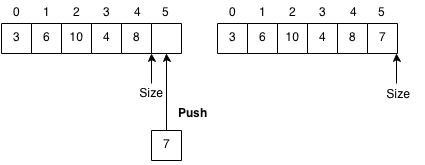
\includegraphics[width=\maxwidth{\textwidth}]{vector2.png}

\begin{lstlisting}
public void add(int x){
        if(size>=arr.length){
        resize();
    }
    arr[size] = x;
    end++;
}
\end{lstlisting}

\subsection{Pop}

Removes the element at the end of the vector. We decrease the size of the vector and return the last element.

\vspace{5px}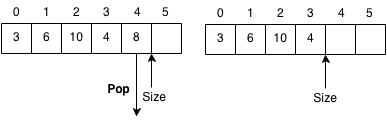
\includegraphics[width=\maxwidth{\textwidth}]{vector4.png}

\begin{lstlisting}
public int pop(){
    if(size==0){
        throw new NoSuchElementException();
    }
    int ret = arr[size];
    size--;
    return ret;
}
\end{lstlisting}

\subsection{Remove}

Removes element at the index idx. It will throw an exception if the index is out of bounds.

We shift everything to the right of the index to the left by one to fill in the missing element.

\vspace{5px}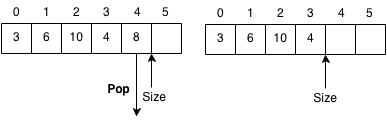
\includegraphics[width=\maxwidth{\textwidth}]{vector4.png}

\begin{lstlisting}
public int remove(int idx){
    if(idx<0||idx>=size){
        throw new ArrayIndexOutOfBoundsException();
    }
    int ret = arr[idx];
    while(idx+1<size){
        arr[idx]=arr[idx+1];
        idx++;
    }
    size--;
    return ret;
}
\end{lstlisting}

\subsection{Get Element}

Returns the element at the specified index. It will throw an exception if the index is out of bounds. Note this function is exactly as the same as in the array

\vspace{5px}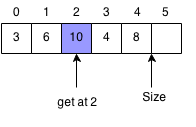
\includegraphics[width=\maxwidth{\textwidth}]{vectorget.png}

\begin{lstlisting}
public int get(int idx){
    if(idx<0||idx>=size){
        throw new ArrayIndexOutOfBoundsException();
    }   
    return arr[idx];
}
\end{lstlisting}

\subsection{Insert Element}

Insert the new number x at the index. We need to make space at the index for the new element so we shift everything to the right of the index by 1.

\vspace{5px}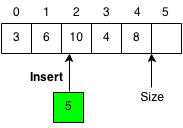
\includegraphics[width=\maxwidth{\textwidth}]{vectorinsert.png}

\vspace{5px}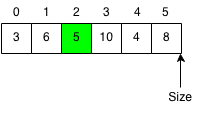
\includegraphics[width=\maxwidth{\textwidth}]{vectorinsert2.png}

\begin{lstlisting}
public void insert(int idx,int x){
    if(idx<0||idx>size){
        throw new ArrayIndexOutOfBoundsException();
    }
    size++;
    if(size>=arr.length){
        resize();
    }
    //Shift elements to the right or idx by 1
    int idx2 = size;
    while(idx2>idx){
        arr[idx2]=arr[idx2-1];
        idx2--;
    }   
    arr[idx] = x;
    }
\end{lstlisting}

\subsection{Exercises}

\begin{enumerate}
\item Implement removeAtIndex(int index) for Vector
\end{enumerate}

    \chapter{ Queue }
        \section{ Queue }
        

A queue is an abstract data type with two functions, pop and push. Removal from the front is called "pop" or "dequeue". Insertion from the back is called "push" or "enqueue". A queue follows a First In First Out (FIFO) structure meaning the first element pushed should be the first element popped and the last element pushed should be the last element popped.

Imagine you are standing in line for a restaurant. Whoever is first in line will be served first and whoever is last in line will be served last. People can be served while more people join the line and the line may get very long because it takes a while to serve one person while more people join the queue. This is called a queue.

Queues are often used for buffer systems, for example a text message service. The messages that arrive at the server first are relayed first and the messages that arrive later are relayed later. If there are too many text messages in the system such that the rate  texts are received overwhelm the number of texts that are sent the buffer may overflow and messages will get dropped. Most of the time this won't happen because the systems are designed to handle large loads, but if there were an emergency that caused everyone to start texting many texts could be dropped.

Example of push:

\vspace{5px}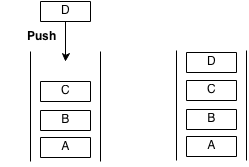
\includegraphics[width=\maxwidth{\textwidth}]{queue.png}

Example of pop:

\vspace{5px}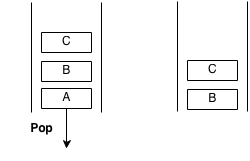
\includegraphics[width=\maxwidth{\textwidth}]{queue2.png}

\subsection{Implementation}

We can implement a queue most efficiently using a linked list because it has an efficient memory allocation.

\vspace{10px}\begin{tabulary}{0.4\linewidth}{|l|l|l|l|l|l|l|l|l|l|l|l|l|l|l|l|l|l|l}\hline


  Implementation &
  Pop &
  Push\\
\hline


  Linked List &
  O(1) &
  O(1)\\

\hline\end{tabulary}

\subsection{Exercises}

\begin{enumerate}
\item Given a list of letters representing instructions where the first instruction is executed, output what the final list should look like after N instructions are executed.

First instruction:

\begin{itemize}
\item A. Add B to the end of the list of instructions
\item B. Do nothing
\item C. Add two A's to the front of the list of instructions
\end{itemize}

Example:

\begin{itemize}
\item ABC
\item BCB
\item CB
\item AAB
\item ABB
\item BBB
\item BB
\item B
\end{itemize}
\end{enumerate}

        \section{ Linked List }
        

Prerequisites: Queue

Source on Github

A linked list is an implementation of a queue that uses a chain of pointers. Instead of storing all the data in a fixed set of memory, we can store each element by itself but have a pointer from each element to the next element. A pointer is something that holds the memory location of another object.

Imagine you were on a scavenger hunt with lots of treasure chests. You start with a clue to the first chest. Each chest contains a lot of gold (data) but it also contains a clue to the next treasure chest. To get to the fifth chest, you need to visit the first, second, third and fourth chest. This is essentially how a linked list works.

\vspace{5px}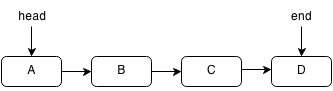
\includegraphics[width=\maxwidth{\textwidth}]{linkedlist.png}

A linked list is similar to an array but it is different such that it is not stored in one block of data. Each element can be stored in a random place in memory but each element contains a pointer to the next element thus forming a chain of pointers. Think of a pointer as a clue to the next chest. Since the elements aren't in a block, accessing an element must be done by traversing the entire linked list by following each pointer to the next. However, this also allows insertion to be done more quickly by simply changing the point of the previous element and setting to the pointer of the current element to the next element. Deletion is also done by taking the previous element and changing its pointer to two elements ahead. In a linked list the links only go forward and you cannot move backward.

A doubly linked list is a linked list that has pointers going backwards as well as forwards.

\vspace{5px}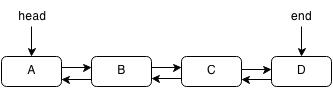
\includegraphics[width=\maxwidth{\textwidth}]{doublelinkedlist.png}

\vspace{10px}\begin{tabulary}{0.4\linewidth}{|l|l|l|l|l|l|l|l|l|l|l|l|l|l|l|l|l|l|l}\hline


  Operation &
  Get &
  Push &
  Delete &
  Insert\\
\hline


  Time Complexity &
  O(n) &
  O(1) &
  O(1) &
  O(1)\\

\hline\end{tabulary}

\subsection{Link Class}

In Java, there already exists a LinkedList class but we will implement our own.

The Link class for each "link" in the Linked List. In each Link we only need the value and location of the previous and next node.

\begin{lstlisting}
class Link{
    int value;
    Link next;
    public Link(int value){
        this.value = value;
        this.next = null;
    }
}
\end{lstlisting}

\subsection{LinkedList Class}

Create the linked list by initializing the starting node as null and setting the size to empty.

\begin{lstlisting}
class LinkedList{
    Link head;
    Link end;
    int size;
    public LinkedList(){
        start = end = null;
        size = 0;
    }
}
\end{lstlisting}

\subsection{Push}

Create a new node with the value given and add it to the end. We have to set the current head previous node to the new node and the new next next to the last node.

\vspace{5px}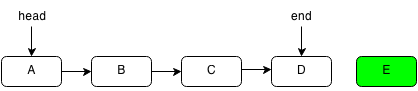
\includegraphics[width=\maxwidth{\textwidth}]{linkedlistpush.png}

\vspace{5px}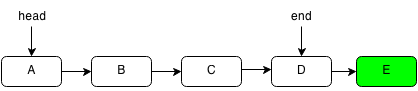
\includegraphics[width=\maxwidth{\textwidth}]{linkedlistpush2.png}

\vspace{5px}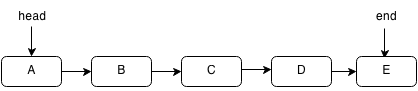
\includegraphics[width=\maxwidth{\textwidth}]{linkedlistpush3.png}

\begin{lstlisting}
/*
 * Adds new node to head of linked list
 */
public void push(int value){
    Link newLink = new Link(value);
    if(size==0){
        head = end = newLink;
    }else{
        end.next = newLink;
        end = newLink;
    }
    size++;
}
\end{lstlisting}

\subsection{Pop}

Pops off the node at the head.

\vspace{5px}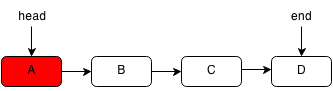
\includegraphics[width=\maxwidth{\textwidth}]{linkedlistpop.png}

\vspace{5px}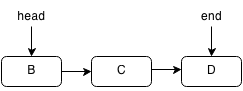
\includegraphics[width=\maxwidth{\textwidth}]{linkedlistpop2.png}

\begin{lstlisting}
/*
 * Adds new node to head of linked list
 */
public int pop(){
    if(head==null){
        throw new NoSuchElementException();
    }
    int ret = head.value;
    head = head.next;
    size--;
    if(size==0){
        end = null;
    }
    return ret;
}
\end{lstlisting}

\subsection{Get}

Get retrieves the value at the specified index. We have to loop through the entire list to get the index we want because the nodes are not in the same block of memory.

\vspace{5px}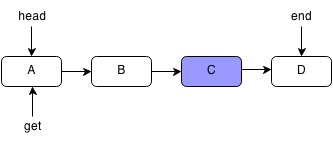
\includegraphics[width=\maxwidth{\textwidth}]{linkedlistget.png}

\vspace{5px}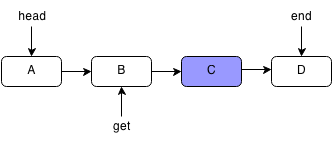
\includegraphics[width=\maxwidth{\textwidth}]{linkedlistget2.png}

\vspace{5px}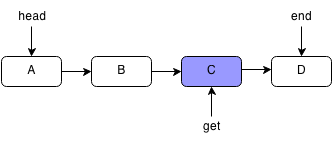
\includegraphics[width=\maxwidth{\textwidth}]{linkedlistget3.png}

\begin{lstlisting}
/*
* Gets the value at index
*/
public int get(int index){
    int i = 0;
    Link curNode = head;
    while(curNode!=null){
        if(index==i){
            return curNode.value;
        }
        curNode = curNode.next;
        i++;
    }
    throw new NoSuchElementException();
}
\end{lstlisting}

\subsection{Delete}

To delete the current node we set the previous node next link to the link after.

\vspace{5px}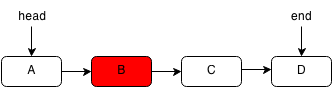
\includegraphics[width=\maxwidth{\textwidth}]{linkedlistrem.png}

\vspace{5px}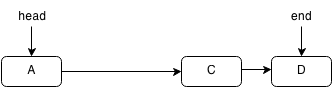
\includegraphics[width=\maxwidth{\textwidth}]{linkedlistrem2.png}

\begin{lstlisting}
/*
 * Deletes node after specified
 */
public void deleteNext(Link node){
    if(node.next==end){
        end = node;
    }
    node.next = node.next.next;
    size--;
}
\end{lstlisting}

\subsection{Exercises}

\begin{enumerate}
\item Implement a doubly linked list.
\item A game is played by always eliminating the kth player from the last elimination and played until one player is left. Given N players each assigned to a number, find the number of the last player.

For example, you have 5 players (1,2,3,4,5) and the 3rd player is eliminated.

\begin{itemize}
\item 1, 2, 3, 4, 5 
\item 1, 2, 4, 5 (1, 2, 3 is eliminated)
\item 2, 4, 5 (4, 5, 1 is eliminated)
\item 2, 4 (2, 4, 5 is eliminated)
\item 2 (2, 4, 2 is eliminated)
\item Player 2 is the last one standing.
\end{itemize}
\item Given two linked lists which may share tails, determine the point at which they converge.
\item Given a node in a doubly linked list, write a function that removes the node from the list. 
\end{enumerate}

    \chapter{ Sets }
        \section{ Sets }
        

Sets are abstract data structures which are able to store and keep track of unique values.

Imagine you have a grocery list that you use to keep track of things you need to buy. You want to make sure there are no duplicate items in the list, you can add items to the list and that you can remove items from your list. This structure is similar to what a set does.

Sets have three operations: insertion, deletion and a membership test. Insertion places an element into the set, deletion removes an element from the set and a membership test is checking whether an element exists within the set.

\subsection{Implementation}

\vspace{10px}\begin{tabulary}{0.4\linewidth}{|l|l|l|l|l|l|l|l|l|l|l|l|l|l|l|l|l|l|l}\hline


  Type &
  Membership &
  Insertion &
  Deletion\\
\hline


  Tree Set &
  O(log n) &
  O(log n) &
  O(log n)\\

  Hash Set &
  O(1) &
  O(1) &
  O(1)\\

\hline\end{tabulary}

\subsection{Exercises}

\begin{enumerate}
\item Given a list of words, determine how many of them are anagrams of each other. An anagram is a word that can have its letters scrambled into another word. 

\begin{itemize}
\item For example silent and listen are anagrams but banana and orange are not.
\end{itemize}
\item Given two lists of friends, find the number of mutual friends.
\item Given a list of numbers, find the number of tuples of size 4 that add to 0. 

\begin{itemize}
\item For example in the list (10,5,-1, 3, 4, -6) the tuple of size 4 (-1,3,4-6) adds to 0.
\end{itemize}
\end{enumerate}

        \section{ Hash Set }
        

Prerequisites: Sets, Linked List

Source on Github

Hash sets are sets that use hashes to store elements. A hashing algorithm is an algorithm that takes an element and converts it to a smaller chunk called a hash. For example let our hashing algorithm be (x mod 10). So the hashes of 232, 217 and 19 are 2,7, and 9 respectively.

\vspace{5px}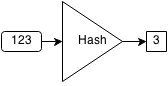
\includegraphics[width=\maxwidth{\textwidth}]{hashcode.png}

For every element in a hash set, the hash is computed and elements with the same hash are grouped together and stored in a linked list. The linked list is called a bucket.

If we want to check if an element already exists within the set, we first compute the hash of the element and then search through the linked list associated with the hash to see if the element is contained.

\vspace{5px}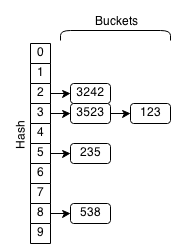
\includegraphics[width=\maxwidth{\textwidth}]{hashset.png}

\vspace{10px}\begin{tabulary}{0.4\linewidth}{|l|l|l|l|l|l|l|l|l|l|l|l|l|l|l|l|l|l|l}\hline


  Operation &
  Membership &
  Insertion &
  Deletion\\
\hline


  Time Complexity &
  O(1) &
  O(1) &
  O(1)\\

\hline\end{tabulary}

\subsection{Implementation}

Let use the example of the hashset of the elements of 3242, 3523, 123, 235 and 538. The hash set looks like this when computed:

\vspace{5px}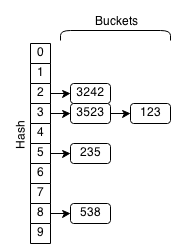
\includegraphics[width=\maxwidth{\textwidth}]{hashset.png}

If we wanted to check if 7238 was in the hash set, we would get the hash (7238 mod 10 = 8). So we get the bucket associated with the hash 8 and we get the list of (538). When we iterate through this short list, we see that 7238 is not a member of the set.

Similarly, if we wanted to insert 7238 into the hash set, we would check if it exists and if it did not we would append the element to the end of the bucket. For deletion we would find 7238 check if it existed in the set and remove it from the bucket.

Hash sets are very efficient in all three set operations if a good hashing algorithm is used. When the objects are that being stored are large then hash sets are effective as a set.

\subsubsection{Class}

Inside our implementation of a hash set we will store the buckets using an array of linked lists, the number of buckets, and the number of elements in the set.

The collision chance is the threshold for resizing the hash set. When the ratio of elements in the set to number of buckets is greater than the threshold, then the chance of collision will be high enough that it will slow down the operations. The lower this ratio, the better performing a hash set will be.

\begin{lstlisting}
public class HashSet {

    public LinkedList<Integer>[] buckets;
    public int bucketsSize = 10;
    public int size = 0;
    public static final double COLLISION_CHANCE = 0.3;
    
    public HashSet(){
        buckets = new LinkedList[10];
        for(int i=0;i<bucketsSize;i++){
            buckets[i] = new LinkedList<Integer>();
        }
        size = 0;
    }
\end{lstlisting}

\subsubsection{Hash code}

The hash code is the result of the hashing algorithm for an element. In our hash set implementation, we will use a simple hash: modulus of the integer by the number of buckets.

\vspace{5px}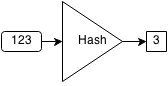
\includegraphics[width=\maxwidth{\textwidth}]{hashcode.png}

For the most part if the numbers are all random then the hash function is fine. However, if the number of buckets was 10 and we added the elements 20,30,40,50,60,70, they will all end up in the same bucket and results in poor performance.

\begin{lstlisting}
public int getHash(int x,int hashSize){
    return x % hashSize;
}
\end{lstlisting}

\subsubsection{Resize}

A hash set must be able to resize. When the ratio of number of elements to number of buckets, the chance of collision will increase more and more. So we must able to resize the number of buckets to support the number of elements to lower the chance of collision.

To resize efficiently, we can create two times the number of buckets and set them to empty and then insert all the elements in the old buckets to the new buckets.

\begin{lstlisting}
public void resize(){
    int newBucketsSize = bucketsSize*2;
    LinkedList<Integer>[] newBuckets = new LinkedList[newBucketsSize];
    for(int i=0;i<newBucketsSize;i++){
        newBuckets[i] = new LinkedList<Integer>();
    }
    for(int i=0;i<bucketsSize;i++){
        for(Integer y:buckets[i]){
            int hash = getHash(y,newBucketsSize);
            newBuckets[hash].push(y);
        }
    }
    buckets = newBuckets;
    bucketsSize = newBucketsSize;
}
\end{lstlisting}

\subsubsection{Insert}

To insert an element in a hash set, we get the hash code from our hashing algorithm and insert the element into the corresponding bucket.

\vspace{5px}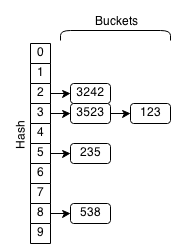
\includegraphics[width=\maxwidth{\textwidth}]{hashset.png}

\vspace{5px}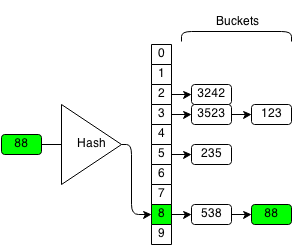
\includegraphics[width=\maxwidth{\textwidth}]{hashsetinsert.png}

The function will return method or not the operation was successful. If the bucket already contains the element the operation will stop because we do not want to add duplicate elements into the set. If the bucket does not contain the element, we will insert it into the bucket and the operation is successful.

\begin{lstlisting}
public boolean insert(int x){
    int hash = getHash(x,bucketsSize);
        
    LinkedList<Integer> curBucket = buckets[hash];
    if(curBucket.contains(x)){
        return false;
    }
    curBucket.push(x);
    if( (float)size/bucketsSize>COLLISION_CHANCE){
        resize();
    }
    size++;
    return true;
}
\end{lstlisting}

\subsubsection{Contains}

To check if a hash set contains an element, we get the hash code from our hashing algorithm and check if the corresponding bucket contains the element.

\vspace{5px}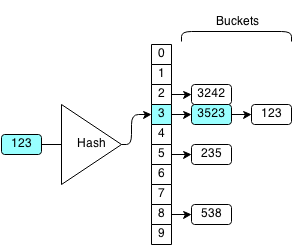
\includegraphics[width=\maxwidth{\textwidth}]{hashsetcontains.png}

\vspace{5px}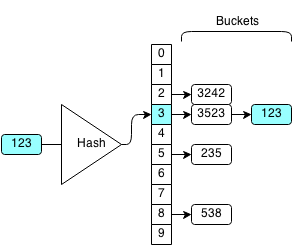
\includegraphics[width=\maxwidth{\textwidth}]{hashsetcontains2.png}

\vspace{5px}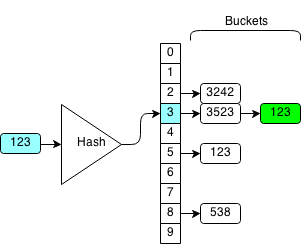
\includegraphics[width=\maxwidth{\textwidth}]{hashsetcontains3.png}

\begin{lstlisting}
public boolean contains(int x){
    int hash = getHash(x,bucketsSize);
    LinkedList<Integer> curBucket = buckets[hash];
    return curBucket.contains(x);
}
\end{lstlisting}

\subsubsection{Remove}

To remove an element from a hash set, we get the hash code from our hashing algorithm and remove the element from the corresponding bucket.

The function will return whether or not the operation was successful. If the bucket contains the element we can remove it from the linked list and the operation is successful. If the element is not in the bucket then the operation fails because we cannot remove something that is not there.

\vspace{5px}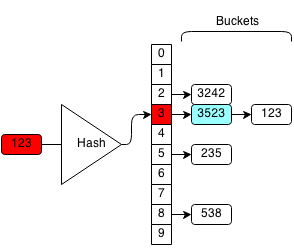
\includegraphics[width=\maxwidth{\textwidth}]{hashsetrem.png}

\vspace{5px}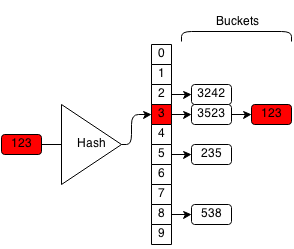
\includegraphics[width=\maxwidth{\textwidth}]{hashsetrem2.png}

\vspace{5px}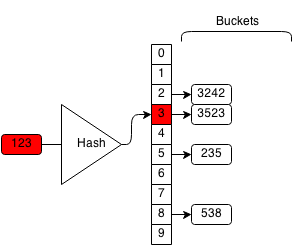
\includegraphics[width=\maxwidth{\textwidth}]{hashsetrem3.png}

\begin{lstlisting}
public boolean remove(int x){
    int hash = getHash(x,bucketsSize);
    
    LinkedList<Integer> curBucket = buckets[hash];
    if(curBucket.remove((Integer)x)){
        return true;
    }
    return false;
}
\end{lstlisting}

\subsection{Exercises}

\begin{enumerate}
\item Try to come up with a better hashing algorithm
\item Calculate the probability of a collision occurring given the number of buckets and number of elements in the hash set
\item Given an array of numbers, find the number of pairs of numbers that sum to 0.
\item Given an array of numbers and a number A, find the number of pairs of numbers that sum to A.
\item Given an array of numbers and a number A, find the number of quadruples that sum to A.
\end{enumerate}

        \section{ Binary Search Tree }
        

A binary search tree is a  binary tree with special properties. The left children of a node will always be less than the node and the right children of a node will always be more than the node. It has a recursive structure such that every subtree is also a binary search tree.

\vspace{5px}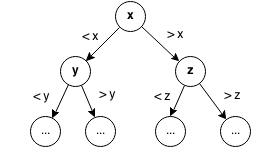
\includegraphics[width=\maxwidth{\textwidth}]{bstcompare.png}

Example:

\vspace{5px}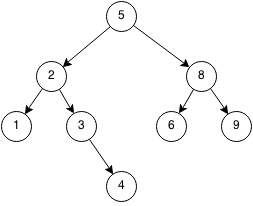
\includegraphics[width=\maxwidth{\textwidth}]{bst.png}

\vspace{10px}\begin{tabulary}{0.4\linewidth}{|l|l|l|l|l|l|l|l|l|l|l|l|l|l|l|l|l|l|l}\hline


  Operation &
  Membership &
  Insertion &
  Deletion\\
\hline


  Time Complexity &
  O(log n) &
  O(log n) &
  O(log n)\\

\hline\end{tabulary}

\subsubsection{Prerequisites}

\begin{itemize}
\item Set
\item Binary Tree
\end{itemize}

\subsection{Implementation}

In a binary search tree, everything to the left of a node is smaller than that node and everything to the right of that node is greater than that node.

\vspace{5px}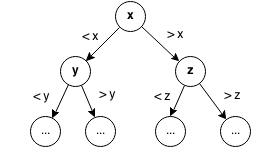
\includegraphics[width=\maxwidth{\textwidth}]{bstcompare.png}

\vspace{5px}\includegraphics[width=\maxwidth{\textwidth}]{bst.png}

This implementation of a binary search will be unbalanced. For a balanced binary search tree, see AVL trees and Red Black trees.

\subsubsection{Class}

A Node is a node in our tree set. Each node will contain a left subtree, a right subtree, the parent of the tree and the value stored at that node. It is unnecessary to store the parent but for this implementation it will be easier to keep track of the parent.

replaceChild replaces the left or right child node specified with the replacement node.

\begin{lstlisting}
public class Node {
    int value;
    Node left;
    Node right;
    Node parent;
    public Node(int val,Node parent){
        this.value = val;
        this.left = null;
        this.right = null;
        this.parent = parent;
    }
    public void replaceChild(Node child,Node replacement){
        if(left==child){
            left = replacement;
            if(replacement!= null){
                replacement.parent = this;
            }
        }
        if(right==child){
            right = replacement;
            if(replacement!= null){
                replacement.parent = this;
            }
        }
    }
}
\end{lstlisting}

In our class we will store the number of element in the set and the root of the tree. From the root of the tree we can traverse the rest of the tree.

\begin{lstlisting}
public class TreeSet {

    int size;
    Node root;
    
    public TreeSet(){
        size = 0;
        root = null;
    }
\end{lstlisting}

\subsubsection{Insert}

To insert an element in the tree set we search for the element that we are trying to insert. If it is already there then the operation fails because sets contain unique elements. Otherwise we will insert the new element into the set.

\vspace{5px}\includegraphics[width=\maxwidth{\textwidth}]{bstinsert.png}

\vspace{5px}\includegraphics[width=\maxwidth{\textwidth}]{bstinsert2.png}

\vspace{5px}\includegraphics[width=\maxwidth{\textwidth}]{bstinsert3.png}

\vspace{5px}\includegraphics[width=\maxwidth{\textwidth}]{bstinsert4.png}

\begin{lstlisting}
public boolean insert(int x){
    if(root==null){
        root = new Node(x,null);
        size = 1;
        return true;
    }
    Node curTree = root;
    while(curTree != null){
        if(x == curTree.value){
            return false;
        }else if(x < curTree.value){
            if(curTree.left == null){
                curTree.left =  new Node(x,curTree);
                size++;
                return true;
            }
            curTree = curTree.left;
        }else {
            if(curTree.right == null){
                curTree.right = new Node(x,curTree);
                size++;
                return true;
            }
            curTree = curTree.right;
        }
    }
    return false;
}
\end{lstlisting}

\subsubsection{Contains}

To check if the tree set contains an element, we search for it in the binary tree by starting at the root. If the number is less than the current, we search the left child. If the number if greater than the current, we search the right child.

\vspace{5px}\includegraphics[width=\maxwidth{\textwidth}]{bstcontains.png}

\vspace{5px}\includegraphics[width=\maxwidth{\textwidth}]{bstcontains2.png}

\vspace{5px}\includegraphics[width=\maxwidth{\textwidth}]{bstcontains3.png}

\vspace{5px}\includegraphics[width=\maxwidth{\textwidth}]{bstcontains4.png}

We return true if it exists and false otherwise.

\begin{lstlisting}
public boolean contains(int x){
    Node curTree = root;
    while(curTree!=null){
        if(x==curTree.value){
            return true;
        }else if(x<curTree.value){
            curTree = curTree.left;
        }else{
            curTree = curTree.right;
        }
    }
    return false;
}
\end{lstlisting}

\subsubsection{Remove}

Removing an element is a much more complex because we need to maintain the tree structure of the tree set when removing elements. First we locate the element that we want to remove. If the element is not there then the operation failed and we return false. If the element is there then are three cases we need to consider.

\vspace{5px}\includegraphics[width=\maxwidth{\textwidth}]{bst-rem.png}

Case 1: Node is a leaf node

\vspace{5px}\includegraphics[width=\maxwidth{\textwidth}]{bst-rem-case11.png}

If the node we want to remove is the leaf node, we can simply remove it.

\vspace{5px}\includegraphics[width=\maxwidth{\textwidth}]{bst-rem-case12.png}

Case 2: Node has one child

\vspace{5px}\includegraphics[width=\maxwidth{\textwidth}]{bst-rem-case21.png}

If the node we want to remove has a child, we can replace that node with its' only child.

\vspace{5px}\includegraphics[width=\maxwidth{\textwidth}]{bst-rem-case22.png}

Case 3: Node has two children

\vspace{5px}\includegraphics[width=\maxwidth{\textwidth}]{bst-rem-case31.png}

We need to replace the node with the rightmost of the left subtree or the leftmost of the right subtree to maintain the order.

\vspace{5px}\includegraphics[width=\maxwidth{\textwidth}]{bst-rem-case32.png}

It does not matter which side we pick so we will use the rightmost of the left subtree. First we copy the value of the rightmost of the left subtree into the node that will be deleted.

\vspace{5px}\includegraphics[width=\maxwidth{\textwidth}]{bst-rem-case33.png}

Then we replace the rightmost of the left subtree with its left subtree.

\vspace{5px}\includegraphics[width=\maxwidth{\textwidth}]{bst-rem-case34.png}

\begin{lstlisting}
public boolean remove(int x){
    //Get node to remove
    Node curNode = root;
    while(curNode!=null){
        if(x==curNode.value){
            break;
        }else if(x<curNode.value){
            curNode = curNode.left;
        }else{
            curNode = curNode.right;
        }
    }
    if(curNode==null){
        return false;
    }
    //Case 1: leaf node
    if(curNode.left==null \&\& curNode.right==null){
        //if root
        if(curNode==root){
            this.root = null;
        }else{
            curNode.parent.replaceChild(curNode,null);
        }
    }
    //Case 2: one child
    else if(curNode.left==null){
        //If root
        if(curNode==root){
            root = curNode.right;
            root.parent = null;
        }else {
            curNode.parent.replaceChild(curNode,curNode.right);
        }
    }
    else if(curNode.right==null){
        //If root
        if(curNode==root){
            root = curNode.left;
            root.parent = null;
        }else {
            curNode.parent.replaceChild(curNode,curNode.left);
        }
    }
    //Case 3: two children
    else {
        //Get rightmost of left subtree
        Node rightmost = curNode.left;
        while(rightmost.right!=null){
            rightmost = rightmost.right;
        }
        curNode.value = rightmost.value;
        rightmost.parent.replaceChild(rightmost, rightmost.left);
    }
    size--;
    return true;
}
\end{lstlisting}

\subsubsection{Print Tree}

Since tree sets are stored as a binary search tree, we can print the elements in order.

\begin{lstlisting}
public String dfs(Node curTree){
    if(curTree == null)return "";
    String ret = "";
    ret += dfs(curTree.left);
    ret += curTree.value;
    ret += ",";
    ret += dfs(curTree.right);
    return ret;
}
    
public String toString(){
    String ret = "";
    if(root!=null){
        ret += dfs(root);
    }
    return ret.substring(0,ret.length()-1);
}
\end{lstlisting}

\subsection{Exercises}

\begin{enumerate}
\item Write a function to determine if a binary tree is a binary search tree
\end{enumerate}

        \section{ Tree Set }
        

Prerequeisites: Sets, Binary Search Tree

Source on Github

A tree set is a set which stores the values in a binary search tree. To store elements in a tree set, they must be able to be sorted by a property. To insert an element, it is added to the binary tree. To delete an element, it is removed from the binary tree. To check for membership, we do a binary search for the element in the binary tree.

The advantage of tree sets is that they are maintained in a sorted order.

\vspace{5px}\includegraphics[width=\maxwidth{\textwidth}]{bst.png}

\vspace{10px}\begin{tabulary}{0.4\linewidth}{|l|l|l|l|l|l|l|l|l|l|l|l|l|l|l|l|l|l|l}\hline


  Operation &
  Membership &
  Insertion &
  Deletion\\
\hline


  Time Complexity &
  O(log n) &
  O(log n) &
  O(log n)\\

\hline\end{tabulary}

\subsection{Implementation}

Tree Sets are implemented using binary search trees.

\subsection{Exercises}

\begin{enumerate}
\item Given a list of names, output all the unique names in alphabetical order
\end{enumerate}

    \chapter{ Maps }
        \section{ Maps }
        

Prerequisites: Sets

A map is an abstract data type that stores key-value pairs.

Imagine you had a English dictionary. If you look up a word, you can find it's definition and read it out. For example if you looked up the word 'cat' in the English dictionary, you would look through the dictionary alphabetically until you found the word 'cat' and then you would look at the definition: 'a feline animal'. If you really wanted to, you could also add your own words into the dictionary and the definitions of your words. This type of structure is called a map.

Maps (also called dictionaries) are abstract data types that store pairs of key-values and can be used to look up values from the keys. The keys are like the words in an English dictionary and the definitions can be seen as the values. Maps are able to support insertion of key-value pairs, retrieve values from keys, and delete key-value pairs.

\subsection{Implementation}

\vspace{10px}\begin{tabulary}{0.4\linewidth}{|l|l|l|l|l|l|l|l|l|l|l|l|l|l|l|l|l|l|l}\hline


  Type &
  Get &
  Insertion &
  Deletion\\
\hline


  Tree Map &
  O(log n) &
  O(log n) &
  O(log n)\\

  Hash Map &
  O(1) &
  O(1) &
  O(1)\\

\hline\end{tabulary}

\subsection{Exercises}

\begin{enumerate}
\item Given a list of N strings, output the strings in alphabetical order and the number of times they appear in the list.
\item Given a mapping of a id to a name, output the ids in order by lexicographical name.
\end{enumerate}

        \section{ Hash Map }
        

Prerequisites: Map, Hash Set



Hash maps are maps that use hash sets to store the keys.

\subsection{Implementation}

Here is a Java implementation of a hash map which is a modified version of a hash set.

\subsubsection{Class}

Inside our implementation of a hash map we will store the buckets using an array of linked lists, the number of buckets, and the number of elements in the set.

The collision chance is the threshold for resizing the hash set. When the ratio of elements in the set to number of buckets is greater than the threshold, then the chance of collision will be high enough that it will slow down the operations. The lower this ratio, the better performing a hash set will be.

\begin{lstlisting}
public class HashMap {

    public LinkedList<Pair>[] buckets;
    public int bucketsSize = 10;
    public int size = 0;
    public static final double COLLISION_CHANCE = 0.3;
    
    public HashMap(){
        buckets = new LinkedList[10];
        for(int i=0;i<bucketsSize;i++){
            buckets[i] = new LinkedList<Pair>();
        }
        size = 0;
    }
}
\end{lstlisting}

\subsubsection{Hash}

The hash code is the result of the hashing algorithm for an element. In our hash set implementation, we will use a simple hash: modulus of the integer by the number of buckets.

For the most part if the numbers are all random then the hash function is fine. However, if the number of buckets was 10 and we added the elements 20,30,40,50,60,70, they will all end up in the same bucket and results in poor performance.

\begin{lstlisting}
public int getHash(int x,int hashSize){
    return x % hashSize;
}
\end{lstlisting}

\subsubsection{Resize}

A hash map must be able to resize. When the ratio of number of elements to number of buckets, the chance of collision will increase more and more. So we must able to resize the number of buckets to support the number of elements to lower the chance of collision.

To resize efficiently, we can create two times the number of buckets and set them to empty and then insert all the elements in the old buckets to the new buckets.

\begin{lstlisting}
public void resize(){
    int newBucketsSize = bucketsSize*2;
    LinkedList<Pair>[] newBuckets = new LinkedList[newBucketsSize];
    for(int i=0;i<newBucketsSize;i++){
        newBuckets[i] = new LinkedList<Pair>();
    }
    for(int i=0;i<bucketsSize;i++){
        for(Pair p:buckets[i]){
            int hash = getHash(p.key,newBucketsSize);
            newBuckets[hash].push(p);
        }
    }
    buckets = newBuckets;
    bucketsSize = newBucketsSize;
}
\end{lstlisting}

\subsubsection{Insert}

To insert an element in a hash set, we get the hash code from our hashing algorithm and insert the element into the corresponding bucket.

The function will return method or not the operation was successful. If the bucket already contains the element the operation will stop because we do not want to add duplicate elements into the set. If the bucket does not contain the element, we will insert it into the bucket and the operation is successful.

\begin{lstlisting}
public boolean insert(Pair p){
    int hash = getHash(p.key,bucketsSize);
    
    LinkedList<Pair> curBucket = buckets[hash];
    if(curBucket.contains(p.key)){
        return false;
    }
    curBucket.push(p);
    if( (float)size/bucketsSize>COLLISION_CHANCE){
        resize();
    }
    size++;
    return true;
}
\end{lstlisting}

\subsubsection{Get}

To get the value from a hash set from a key, we get the hash code from our hashing algorithm of the key and find the key-value pair in the corresponding bucket.

\begin{lstlisting}
public Pair get(int key){
    int hash = getHash(key,bucketsSize);
    LinkedList<Pair> curBucket = buckets[hash];
    for(Pair p:curBucket){
        if(p.key==key){
            return p;
        }
    }
    return null;
}
\end{lstlisting}

\subsubsection{Remove}

To remove an element from a hash set, we get the hash code from our hashing algorithm and remove the element from the corresponding bucket.

The function will return whether or not the operation was successful. If the bucket contains the element we can remove it from the linked list and the operation is successful. If the element is not in the bucket then the operation fails because we cannot remove something that is not there.

\begin{lstlisting}
public boolean remove(int key){
    int hash = getHash(key,bucketsSize);
    
    LinkedList<Pair> curBucket = buckets[hash];
    for(Pair p: curBucket){
        if(p.key==key){
            curBucket.remove(p);
            return true;
        }
    }
    return false;
}
\end{lstlisting}

\subsection{Exercises}

\begin{enumerate}
\item Create a hash map for the English dictionary (word as keys, definition as value). You will need to create a hash function for strings.
\end{enumerate}

        \section{ Tree Map }
        

Prerequisites: Tree Set, Map

A tree map is a map that stores the key value pairs in a tree set.

\vspace{10px}\begin{tabulary}{0.4\linewidth}{|l|l|l|l|l|l|l|l|l|l|l|l|l|l|l|l|l|l|l}\hline


  Operation &
  Membership &
  Insertion &
  Deletion\\
\hline


  Complexity &
  O(log n) &
  O(log n) &
  O(log n)\\

\hline\end{tabulary}

\subsection{Implementation}

Here is a Java implementation of a tree map:

\vspace{5px}\includegraphics[width=\maxwidth{\textwidth}]{bst.png}

\subsubsection{Class}

A pair is a key with a value. In this implementation we will use the value as a string.

\begin{lstlisting}
class Pair{
    int key;
    String value;
    public Pair(int key,String value){
        this.key = key;
        this.value = value;
    }
}
\end{lstlisting}

A node is a node contained in the binary search tree. The node must store the child nodes and for simplicity of the implementation, we will store the parent node as well. Each node will also have a key value pair associated with it.

\begin{lstlisting}
class Node{
    Pair pair;
    Node left;
    Node right;
    Node parent;
    public Node(Pair p){
        this.pair = p;
        this.left = null;
        this.right = null;
        this.parent = null;
    }
    public void replaceChild(Node child,Node replacement){
        if(left==child){
            left = replacement;
                if(replacement!= null){
                    replacement.parent = this;
                }
            }
            if(right==child){
                right = replacement;
                if(replacement!= null){
                    replacement.parent = this;
                }
            }
        }
    }
}
\end{lstlisting}

In our tree map, we will store the root node (ancestor of all nodes) and the number of numbers.

\begin{lstlisting}
public class TreeMap {

    int size;
    Node root;
    
    public TreeMap(){
        size = 0;
        root = null;
    }
}
\end{lstlisting}

\subsubsection{Insert}

To insert a key-value pair into the tree set, we first find where the key should be. If the key already exists,

\begin{lstlisting}
public boolean insert(Pair p){
    if(root==null){
        root = new Node(p);
        return true;
    }
    Node curTree = root;        
    while(curTree != null){
        if(p.key == curTree.pair.key){
            return false;
        }else if(p.key < curTree.pair.key){
            if(curTree.left == null){
                Node newTree = new Node(p);
                newTree.parent = curTree;
                curTree.left = newTree;
                return true;
            }
            curTree = curTree.left;
        }else {
            if(curTree.right == null){
                Node newTree = new Node(p);
                newTree.parent = curTree;
                curTree.right = newTree;
                return true;
            }
            curTree = curTree.right;
        }
    }
    return false;
}
\end{lstlisting}

\subsubsection{Get}

To get the value from a key stored in a tree set, we binary search for the key and then retrieve the key-value pair located at the node.

\begin{lstlisting}
public Pair get(int key){
    Node curTree = root;
    while(curTree!=null){
        if(key==curTree.pair.key){
            return curTree.pair;
        }else if(key<curTree.pair.key){
            curTree = curTree.left;
        }else{
            curTree = curTree.right;
        }
    }
    return null;
}
\end{lstlisting}

\subsubsection{Remove}

Removing an element is a much more complex because we need to maintain the tree structure of the tree set when removing elements. First we locate the element that we want to remove. If the element is not there then the operation failed and we return false. If the element is there then are three cases we need to consider.

\vspace{5px}\includegraphics[width=\maxwidth{\textwidth}]{bst-rem.png}

Case 1: Node is a leaf node

\vspace{5px}\includegraphics[width=\maxwidth{\textwidth}]{bst-rem-case11.png}

If the node we want to remove is the leaf node, we can simply remove it.

\vspace{5px}\includegraphics[width=\maxwidth{\textwidth}]{bst-rem-case12.png}

Case 2: Node has one child

\vspace{5px}\includegraphics[width=\maxwidth{\textwidth}]{bst-rem-case21.png}

If the node we want to remove has a child, we can replace that node with its' only child.

\vspace{5px}\includegraphics[width=\maxwidth{\textwidth}]{bst-rem-case22.png}

Case 3: Node has two children

\vspace{5px}\includegraphics[width=\maxwidth{\textwidth}]{bst-rem-case31.png}

We need to replace the node with the rightmost of the left subtree or the leftmost of the right subtree to maintain the order.

\vspace{5px}\includegraphics[width=\maxwidth{\textwidth}]{bst-rem-case32.png}

It does not matter which side we pick so we will use the rightmost of the left subtree. First we copy the value of the rightmost of the left subtree into the node that will be deleted.

\vspace{5px}\includegraphics[width=\maxwidth{\textwidth}]{bst-rem-case33.png}

Then we replace the rightmost of the left subtree with its left subtree.

\vspace{5px}\includegraphics[width=\maxwidth{\textwidth}]{bst-rem-case34.png}

\begin{lstlisting}
public boolean remove(int key){
    //Get node to remove
    Node curNode = root;
    while(curNode!=null){
        if(key==curNode.pair.key){
            break;
        }else if(key<curNode.pair.key){
            curNode = curNode.left;
        }else{
            curNode = curNode.right;
        }
    }
    if(curNode==null){
        return false;
    }
    //Case 1: leaf node
    if(curNode.left==null \&\& curNode.right==null){
        //if root
        if(curNode==root){
            this.root = null;
        }else{
            curNode.parent.replaceChild(curNode,null);
        }
    }
    //Case 2: one child
    else if(curNode.left==null){
        //If root
        if(curNode==root){
            root = curNode.right;
            root.parent = null;
        }else {
            curNode.parent.replaceChild(curNode,curNode.right);
        }
    }
    else if(curNode.right==null){
        //If root
        if(curNode==root){
            root = curNode.left;
            root.parent = null;
        }else {
            curNode.parent.replaceChild(curNode,curNode.left);
        }
    }
    //Case 3: two children
    else {
        //Get rightmost of left subtree
        Node rightmost = curNode.left;
        while(rightmost.right!=null){
            rightmost = rightmost.right;
        }
        curNode.pair = rightmost.pair;
        rightmost.parent.replaceChild(rightmost, rightmost.left);
    }
    size--;
    return true;
}
\end{lstlisting}

\subsection{Exercises}

\begin{enumerate}
\item Given a list of N numbers, output the first M unique numbers.
\end{enumerate}

    \chapter{ Priority Queue }
        

Prerequisites: Queue, Heap

A priority queue is a queue that takes elements which have the highest priority first. This is either the maximum or minimum property for all elements.

Consider a waiting list for lung donors. The patients are given a score when they are placed on the waiting list by how much they need a lung based on their whether they smoke, risk factors, age, expected time left etc. When a lung is available, the patient with the highest score will get removed from the waiting list. During this time, more patients could be added to the queue. The behaviour is similar to a queue but instead of the first person getting in the queue getting a lung first, the person with the highest score will get it. This means that if Sam has a score of 60 and gets placed in the queue after Bob who has a score of 40, Sam will get the lung first even though Bob was in the queue before him.

A priority queue is an abstract data structure with two operations: push and pop. Push adds an element into the priority queue and pop removes the highest or lowest element.

A priority queue is usually implemented as a heap because it is the most efficient because of its structure.

\subsection{Implementation}

\vspace{10px}\begin{tabulary}{0.4\linewidth}{|l|l|l|l|l|l|l|l|l|l|l|l|l|l|l|l|l|l|l}\hline


  Implementation &
  Push &
  Pop\\
\hline


  Heap &
  O(log n) &
  O(log n)\\

\hline\end{tabulary}

\subsection{Applications}

Priority queues are very efficient in its opertions O(log n) and it is used in many other algorithms such as:

\begin{itemize}
\item Dijkstra's
\item Prim's
\item Kruskal
\item Line Sweeping
\end{itemize}

\subsection{Exercises}

\begin{enumerate}
\item Given a list of N numbers, find the M largest numbers. (Note you can do better than O(N log N))
\item Given N lists of N numbers, find the N largest numbers.
\end{enumerate}

        \section{ Heap }
        

Prerequisites: Queue



Heaps are data structures that are able to pop the maximum or minimum value or push a value very quickly. Heaps are implemented as trees which have the property that a parent node must either be greater than all the elements in its left and right subtrees (a max heap) or less than all the elements in its left and right subtrees (a min heap). Priority queue's are most efficiently implemented as heaps. This guarantees that the maximum or minimum element is the root node.

Heaps store their data level by level in a binary tree. This allows us to store heaps in an array. The root index is 0. For every node, the left index can be found by using the formula 2=ind+1 and the right index can be found by using the formula 2=ind + 2. The parent of a node can be found by integer division with (ind-1)/2.

\begin{lstlisting}
root = 0
left = index * 2 + 1
right = index * 2 + 2
parent = (index-1)/2
\end{lstlisting}

Indexes of a heap

\vspace{5px}\includegraphics[width=\maxwidth{\textwidth}]{maxheap2.png}

Example Heap:

\vspace{5px}\includegraphics[width=\maxwidth{\textwidth}]{maxheap.png}

A heap has two operations: push and pop. Pushing an element into a heap adds it into the heap and the heap needs to ensure that the properties of the heap still hold. Popping removes an element from the top of the heap and the heap needs to ensure that the properties of the heap still hold.

\vspace{10px}\begin{tabulary}{0.4\linewidth}{|l|l|l|l|l|l|l|l|l|l|l|l|l|l|l|l|l|l|l}\hline


  Operation &
  Heapify &
  Resize &
  Push &
  Pop\\
\hline


  Time Complexity &
  O(n) &
  O(n) &
  O(log n) &
  O(log n)\\

\hline\end{tabulary}

\subsection{Implementation}

Here is an implementation of a max heap. A heap needs to be able to resize, push an element and pop an element.

\subsubsection{Class}

\begin{lstlisting}
public class Heap {

    public int[] arr;
    public int size;
    
    public Heap(int startSize){
        arr = new int[startSize];
        size = 0;
    }
}
\end{lstlisting}

\subsubsection{Heapify}

Heapify takes a random array of N elements and transforms it into a heap. The runtime of heapify is O(N).

\begin{lstlisting}
public void heapify(int arr[]){
    this.arr = arr;
    for(int i=0;i<Math.floor(arr.length/2.0);i++){
        int idx = i;
        while(idx<size){
            int left = idx*2+1;
            int right = idx*2+2;
            if(left<size \&\& arr[left]>arr[idx]){
                int swap = arr[left];
                arr[left] = arr[idx];
                arr[idx] = swap;
                idx = left;
            }else if(right<size \&\& arr[right]>arr[idx]){
                int swap = arr[right];
                arr[right]=arr[idx];
                arr[idx] = swap;
                idx = right;
            }else {
                break;
            }
        }
    }
}
\end{lstlisting}

\subsubsection{Resize}

When the heap gets too full, we can resize it to make it bigger

\begin{lstlisting}
public void resize(){
    int[] newArr = new int[arr.length*2];
    for(int i=0;i<size;i++){
        newArr[i] = arr[i];
    }
    arr = newArr;
}
\end{lstlisting}

\subsubsection{Push}

Pushes the number x into the priority queue. We can do this by adding it to the bottom of the heap and then keep swapping it upwards if it is greater than the parent.

\vspace{5px}\includegraphics[width=\maxwidth{\textwidth}]{maxheap.png}

\vspace{5px}\includegraphics[width=\maxwidth{\textwidth}]{maxheappush.png}

\vspace{5px}\includegraphics[width=\maxwidth{\textwidth}]{maxheappush2.png}

\vspace{5px}\includegraphics[width=\maxwidth{\textwidth}]{maxheappush3.png}

\begin{lstlisting}
public void push(int x){
        
    if(size>=arr.length){
        resize();
    }
    arr[size] = x;
    size++;
    
    //Make sure parent is > child from the last element
    int idx = size-1;
    int parent = (idx-1)/2;
    while(idx>0 \&\& arr[parent]<arr[idx]){
        int swap = arr[parent];
        arr[parent] = arr[idx];
        arr[idx] = swap;
        idx = parent;
        parent = (idx-1)/2;
    }
}
\end{lstlisting}

\subsubsection{Pop}

Popping removes the greatest element in the priority queue by removing the root which is guaranteed to be the greatest as property of a heap. After removing the root, we replace it with the element at the bottom of the heap and we can keep swapping it with its children until the heap property is satisfied.

\vspace{5px}\includegraphics[width=\maxwidth{\textwidth}]{maxheappop.png}

\vspace{5px}\includegraphics[width=\maxwidth{\textwidth}]{maxheappop1.png}

\vspace{5px}\includegraphics[width=\maxwidth{\textwidth}]{maxheappop2.png}

\vspace{5px}\includegraphics[width=\maxwidth{\textwidth}]{maxheappop3.png}

\begin{lstlisting}
public int pop(){
    if(size==0)return 0;
    int ret = arr[0];
    arr[0] = arr[size-1];
    size--;
        
    int idx = 0;
        
    while(idx<size){
        int left = idx*2+1;
        int right = idx*2+2;
        if(left<size \&\& arr[left]>arr[idx]){
            int swap = arr[left];
            arr[left] = arr[idx];
            arr[idx] = swap;
            idx = left;
        }else if(right<size \&\& arr[right]>arr[idx]){
            int swap = arr[right];
            arr[right]=arr[idx];
            arr[idx] = swap;
            idx = right;
        }else {
            break;
        }
    }
}
\end{lstlisting}

\subsection{Applications}

Heaps are very efficient in its opertions O(log n) and it is used in many other algorithms such as:

\begin{itemize}
\item Dijkstra's
\item Prim's
\item Kruskal
\item Line Sweeping
\end{itemize}

\subsection{Exercises}

\begin{enumerate}
\item Implement a min heap
\item Prove heaps work
\end{enumerate}

\part{ Graph Theory }
    

Next: Advanced Graph Theory

Graphs are a set of objects where some pairs of objects  called nodes or verticies are usually connected by links called edges. The nodes here can be seen numbered from 1 to 6. There are edges connecting these various nodes.

\vspace{5px}\includegraphics[width=\maxwidth{\textwidth}]{graph.png}

A undirected graph is a graph where an edge from A to B is the same as the edge from B to A for all edges. The above graph is undirected.

A directed or bidirectional graph is a graph where edges have direction meaning if there is an edge from A to B then there may not be an edge from B to A.

\vspace{5px}\includegraphics[width=\maxwidth{\textwidth}]{digraph.png}

A subgraph is a subset of edges and vertices within a graph.

A directed acyclic graph (DAG) is a graph with no directed cycles (see topological sorting).

A weighted graph is a graph that contains weights or values assigned to each edge or node. Usually these weights act as the cost to reach/use that node.


    \chapter{ Representation }
        

A graph can be represented as a adjacency matrix or a adjacency list.

\subsubsection{Adjacency Matrix}



An adjacency matrix is a method of storing a graph using a two dimensional array. Given n nodes, the adjacency matrix can be stored in a n x n matrix.

Array[i][j] represents the weight between the node i and node j.

Example

\vspace{10px}\begin{tabulary}{0.4\linewidth}{|l|l|l|l|l|l|l|l|l|l|l|l|l|l|l|l|l|l|l}\hline


   &
  1 &
  2 &
  3 &
  4 &
  5 &
  6\\
\hline


  1 &
  0 &
  1 &
  0 &
  0 &
  1 &
  0\\

  2 &
  1 &
  0 &
  1 &
  0 &
  1 &
  0\\

  3 &
  0 &
  1 &
  0 &
  1 &
  0 &
  0\\

  4 &
  0 &
  0 &
  1 &
  0 &
  1 &
  1\\

  5 &
  1 &
  1 &
  0 &
  1 &
  0 &
  0\\

  6 &
  0 &
  0 &
  0 &
  1 &
  0 &
  0\\

\hline\end{tabulary}



\subsubsection{Adjacency List}



Adjacency lists use an array of linked lists to store all the edges. At x, you have a linked list of nodes that connect to 
that node. 1 connects to nodes 2 and 5, 2 connects to 1, 3 and 5 and so forth. O(m) storage where m is number of edges.

\vspace{5px}\includegraphics[width=\maxwidth{\textwidth}]{graph.png}

\vspace{10px}\begin{tabulary}{0.4\linewidth}{|l|l|l|l|l|l|l|l|l|l|l|l|l|l|l|l|l|l|l}\hline


  Node &
  edges\\
\hline


  1 &
  2, 5\\

  2 &
  1 3 5\\

  3 &
  2 4\\

  4 &
  3 5 6\\

  5 &
  1 2 4\\

  6 &
  4\\

\hline\end{tabulary}



        \section{ Adjacency Matrix }
        

An adjacency matrix is a method of storing a graph using a two dimensional array. Given n nodes, the adjacency matrix can be stored in a n x n matrix.

Array[i][j] represents the weight between the node i and node j.

Example

\vspace{10px}\begin{tabulary}{0.4\linewidth}{|l|l|l|l|l|l|l|l|l|l|l|l|l|l|l|l|l|l|l}\hline


   &
  1 &
  2 &
  3 &
  4 &
  5 &
  6\\
\hline


  1 &
  0 &
  1 &
  0 &
  0 &
  1 &
  0\\

  2 &
  1 &
  0 &
  1 &
  0 &
  1 &
  0\\

  3 &
  0 &
  1 &
  0 &
  1 &
  0 &
  0\\

  4 &
  0 &
  0 &
  1 &
  0 &
  1 &
  1\\

  5 &
  1 &
  1 &
  0 &
  1 &
  0 &
  0\\

  6 &
  0 &
  0 &
  0 &
  1 &
  0 &
  0\\

\hline\end{tabulary}

\subsection{Implementation}

\begin{lstlisting}
class edge{
    int weight,source,dest;
    public edge(int source,int dest,int weight){
        this.source = source;
        this.dest = dest;
        this.weight = weight;
    }
}
public static int[][] getAdjMatrix(Vector<edge> edges){
    int n = 0;
    int adjMatrix[][] = new int[n][n];
    
    for(int i=0;i<n;i++)for(int j=0;j<n;j++)adjMatrix[i][j] = 0;
    
    for(int i=0;i<edges.size();i++){
        edge e = edges.get(i);
        adjMatrix[e.source][e.dest] = e.weight;
        adjMatrix[e.dest][e.source] = e.weight;
    }
    return adjMatrix;
}
\end{lstlisting}

        \section{ Adjacency List }
        

Adjacency lists use an array of linked lists to store all the edges. At x, you have a linked list of nodes that connect to 
that node. 1 connects to nodes 2 and 5, 2 connects to 1, 3 and 5 and so forth. O(m) storage where m is number of edges.

\vspace{5px}\includegraphics[width=\maxwidth{\textwidth}]{graph.png}

\vspace{10px}\begin{tabulary}{0.4\linewidth}{|l|l|l|l|l|l|l|l|l|l|l|l|l|l|l|l|l|l|l}\hline


  Node &
  edges\\
\hline


  1 &
  2, 5\\

  2 &
  1 3 5\\

  3 &
  2 4\\

  4 &
  3 5 6\\

  5 &
  1 2 4\\

  6 &
  4\\

\hline\end{tabulary}

    \chapter{ Tree }
        



A tree is a special graph with no cycles. It has the special property that there will be only one path from one node to another node.

\vspace{5px}\includegraphics[width=\maxwidth{\textwidth}]{treegraph.png}

A subtree is a child tree of a tree.

Note that trees have two meanings in computer science. It can either refer to a tree data structure or it can refer to a tree in graph theory.


\subsubsection{Spanning Tree}



A spanning tree of a graph is a connected tree that spans all the nodes of the graph.

A minimum spanning tree is the spanning tree that requires the minimum of some property such as total weight or total edges.

Spanning tree algorithms are essential in networking to ensure no loops occur when sending data through a network.

\vspace{10px}\begin{tabulary}{0.4\linewidth}{|l|l|l|l|l|l|l|l|l|l|l|l|l|l|l|l|l|l|l}\hline


  Algorithm &
  Desc &
  Time &
  Space\\
\hline


  Prim's &
  Using greedy method &
  O(n log n) &
  O(n$^{2}$)\\

  Kruskal &
  Using connected components &
  O(n log n) &
  O(n$^{2}$)\\

\hline\end{tabulary}



        \section{ Prim's }
        Prerequisites:  Priority Queue, Minimum Spanning Tree

A minimum spanning tree is a tree in a graph that connects all the nodes using the smallest cost total cost of edges.

\subsection{Implementation}

Prim's algorithm finds the minimum spanning tree using a greedy fashion. It works as such:

\begin{enumerate}
\item Pick an arbitrary node
\item Find the closest node to that node
\item Find the closest node to the 2 nodes
\item Find the closest node to the 3 nodes
\item ...
\item Find the closest node to n-1 nodes
\end{enumerate}

The closest node is the node with the lowest cost edge to the already connected nodes.

\subsubsection{Example}

\vspace{5px}\includegraphics[width=\maxwidth{\textwidth}]{prim.png}

\vspace{5px}\includegraphics[width=\maxwidth{\textwidth}]{prim1.png}

\vspace{5px}\includegraphics[width=\maxwidth{\textwidth}]{prim2.png}

\vspace{5px}\includegraphics[width=\maxwidth{\textwidth}]{prim3.png}

\vspace{5px}\includegraphics[width=\maxwidth{\textwidth}]{prim4.png}

\vspace{5px}\includegraphics[width=\maxwidth{\textwidth}]{prim5.png}

\vspace{5px}\includegraphics[width=\maxwidth{\textwidth}]{prim6.png}

\vspace{5px}\includegraphics[width=\maxwidth{\textwidth}]{prim7.png}

\subsubsection{Java Code}

In Java, we need to specify a comparison for the Priority Queue to order. We do this by implementing the Comparable class and overriding the compareTo method.

adjList is an adjacency list that is an array of arrays that store the graph.

\begin{lstlisting}

class node implements Comparable<node>{
    int weight,index;
    public node(int weight,int index){
        this.weight = weight;
        this.index = index;
    }
    public int compareTo(node e){
        return weight-e.weight;
    }
}
public static int Prims(Vector<Vector<node>> adjList){
    int cost = 0;
    int n = adjList.size();
    PriorityQueue<node> pq = new PriorityQueue<node>();
    boolean visited[] = new boolean[n];
    for(int i=0;i<n;i++){
        visited[i] = false;
    }
    int inTree = 1;
    visited[0] = true;
    for(int i=0;i<adjList.get(0).size();i++){
        pq.add(adjList.get(0).get(i));
    }
    while(!pq.isEmpty()\&\&inTree<n){
        node cur = pq.poll();
        if(visited[cur.index])continue;
        inTree++;
        visited[cur.index]=true;
        cost+=cur.weight;
        for(int i=0;i<adjList.get(cur.index).size();i++){
            pq.add(adjList.get(cur.index).get(i));          
                 }
    }
    //Graph is not connected
    if(inTree<n)return -1;
    return cost;
}
\end{lstlisting}

\subsection{Applications}

In networking, if a cable company wanted to connect all the houses with the least amount of wiring, the minimum spanning tree can be found that finds the least total cost of wire.

Minimum spanning trees can also be used in generating mazes.

\subsection{Exercises}

\begin{enumerate}
\item Prove that Prim's algorithm works
\item Extends Prim's to output all the edges used
\item Given a weighted graph with n nodes, find the smallest total cost to connect all nodes into 3 separate groups. (A single node can be a group)
\item Same as 3, but a group must contain at least 3 other nodes.
\end{enumerate}

        \section{ Kruskal }
        

Prerequisites:  Sorting, Minimum Spanning Tree

A minimum spanning tree is a tree in a graph that connects all the nodes using the smallest cost total cost of edges.

Kruskal's algorithm finds the minimum spanning tree using connected components.

If implemented efficiently using a priority queue to get the edges with minimum weight or a sorting the edges, the runtime is O(n log n).

\subsection{Implementation}

\begin{enumerate}
\item Uniquely label each node
\item Take the edge with the minimum weight
\item If the edge connects nodes A and B with different labels, all nodes with label B will be labeled with A. Otherwise, throw the edge away
\item Repeat 2-3 until all the nodes have the same label
\end{enumerate}

\subsubsection{Example}

\vspace{5px}\includegraphics[width=\maxwidth{\textwidth}]{kruskal.png}

\vspace{5px}\includegraphics[width=\maxwidth{\textwidth}]{kruskal2.png}

\vspace{5px}\includegraphics[width=\maxwidth{\textwidth}]{kruskal3.png}

\vspace{5px}\includegraphics[width=\maxwidth{\textwidth}]{kruskal4.png}

\vspace{5px}\includegraphics[width=\maxwidth{\textwidth}]{kruskal5.png}

\vspace{5px}\includegraphics[width=\maxwidth{\textwidth}]{kruskal6.png}

\vspace{5px}\includegraphics[width=\maxwidth{\textwidth}]{kruskal7.png}

\subsubsection{Code}

\begin{lstlisting}
class edge implements Comparable<edge>{
    int weight,source,dest;
    public edge(int source,int dest,int weight){
        this.source = source;
        this.dest = dest;
        this.weight = weight;
    }
    public int compareTo(edge e){
        return weight-e.weight;
    }
}
public static int getParent(int parents[],int x){
    if(parents[x]==x)return x;
    parents[x] = getParent(parents,parents[x]);
    return parents[x];
}
public static int Kruskal(Vector<Vector<edge>> adjList){
    int n = adjList.size();
    int parents[] = new int[n];
    for(int i=0;i<n;i++)parents[i] = i;
    int sum = 0;
    
    PriorityQueue<edge> edges = new PriorityQueue<edge>();
    
    for(int i=0;i<n;i++){
        for(int j=0;j<adjList.get(i).size();j++){
            edges.add(adjList.get(i).get(j));
        }
    }
    
    while(!edges.isEmpty()){
        edge e = edges.poll();
        if(getParent(parents,e.source)!=getParent(parents,e.dest)){
            parents[e.source] = getParent(parents,e.dest);
            sum+=e.weight;
        }
    }
    
    return sum;
}
\end{lstlisting}

\subsection{Applications}

\subsection{Exercises}

\begin{enumerate}
\item Prove Kruskal's Algorithm works
\item Extends Kruskals's to output all the edges used
\item Given a weighted graph with n nodes, find the smallest total cost to connect all nodes into 3 separate groups. (A single node can be a group)
\item Same as 3, but a group must contain at least 3 other nodes.
\end{enumerate}

    \chapter{ Shortest Path }
        

The shortest path is defined as a path from one node to another while trying to minimize a certain property (least number of nodes, smallest total weight). However, shortest paths may have negative weights which leads to cycles.

\subsubsection{Algorithms}

\vspace{10px}\begin{tabulary}{0.4\linewidth}{|l|l|l|l|l|l|l|l|l|l|l|l|l|l|l|l|l|l|l}\hline


  Algorithm &
  Desc &
  Time &
  Space &
  Detect cycles?\\
\hline


  Floyd Warshall &
  Computes shortest path between all pairs of nodes &
  O(n$^{3}$) &
  O(n$^{2}$) &
  Yes\\

  Bellman Ford &
  Computes shortest path between a pairs of nodes &
  O(n$^{2}$) &
  O(n) &
  Yes\\

  Dijkstra's &
  Computes shortest path between a pair of nodes using the Greedy method &
  O(n log n) &
  O(n log n) &
  No\\

\hline\end{tabulary}


        \section{ Dijkstra's }
        

Prerequisites:  Shortest Path, Priority Queue, Greedy Algorithm

Dijkstra's is a greedy approach to find the shortest path in a graph with positive weights. It has many useful applications in networking and it can be extended to a variety of problems.

Dijkstra works by beginning at the starting node repeatedly picking the next closest node of those already visited.

If Dijkstra's is implemented using a priority queue, the run time is O(n log n).

If a negative cycle exists within the graph, then the algorithm breaks as it will repeatedly try to take the negative edges. See Bellman Ford to find negative cycles in a graph.

A naive fix for negative cycles would be to offset all edges by the largest negative edge and then subtract it from the resulting total but this does not work. Consider an example where you have start node A and end node B. The first route from A-$>$B has length 2 and the second route has lengths 1,1,-2. Clearly the second route has less cost. If we try to make the length positive by adding all costs by 2, we will have the first path of length 4 and the second path of lengths 3,3,0 and the first route becomes the smallest total cost which is wrong.

\subsection{Implementation}

At each node we visit we keep track of the minimum cost it takes to reach to reach that node from the starting node.

\begin{enumerate}
\item Start at the starting node
\item Find an unvisited node that has the least cost to reach from the visited nodes.
\item Mark that node as visited
\item Repeat until all nodes are visited
\end{enumerate}

When we reach a node for the first time, it will be the shortest path to that node (Try to prove this to yourself).

We first start at the starting node. The distance from the starting node to the starting node is obviously 0.

\vspace{5px}\includegraphics[width=\maxwidth{\textwidth}]{djikstra.png}

From the starting node we have two nodes we can reach. The top node has a cost of 3 to reach and the bottom node has a cost of 5 to reach.

\vspace{5px}\includegraphics[width=\maxwidth{\textwidth}]{djikstra1.png}

We pick the smallest node the reach and we mark it as visited. Once we visit a node, we can guarantee that it is the smallest cost to reach it. The next nodes minimum cost to reach is 10, 5 and 5.

\vspace{5px}\includegraphics[width=\maxwidth{\textwidth}]{djikstra2.png}

We are indifferent to both 5's as they are both the minimum and we can choose either. We mark the node as visited and we find the minimum costs to other nodes which are 5,10,11.

\vspace{5px}\includegraphics[width=\maxwidth{\textwidth}]{djikstra3.png}

We take the next smallest which is 5 and we mark the node as visited. The next costs are 10 and 11.

\vspace{5px}\includegraphics[width=\maxwidth{\textwidth}]{djikstra4.png}

We take the smallest which is 10 and we now only have one last node to reach at a cost of 11.

\vspace{5px}\includegraphics[width=\maxwidth{\textwidth}]{djikstra5.png}

At each node we have the minimum cost to get from the start node to each node.

\vspace{5px}\includegraphics[width=\maxwidth{\textwidth}]{djikstra6.png}

\subsubsection{Java}

Implementation of Dijkstra in Java using a priority queue.

\begin{lstlisting}
class node implements Comparable<node>{
    int weight,index;
    public node(int weight,int index){
        this.weight = weight;
        this.index = index;
    }
    public int compareTo(node e){
        return weight-e.weight;
    }
}

public static int dijkstra(int[][] adjMatrix,int start,int end){
    int n = adjMatrix.length;
    PriorityQueue <node> pq = new PriorityQueue<node>();
    boolean visited[] = new boolean[n];
    for(int i=0;i<n;i++)visited[i] = false;
    pq.add(new node(0,start));
    while(!visited[end] \&\& !pq.isEmpty()){
        node curNode = pq.poll();
    
        if(visited[curNode.index])continue;
        visited[curNode.index] = true;
        if(curNode.index==end){
            return curNode.weight;
        }
        for(int i=0;i<n;i++){
            if(adjMatrix[curNode.index][i]>0 \&\& !visited[i]){
                int newWeight = curNode.weight+adjMatrix[curNode.index][i];
                pq.add(new node(newWeight,i));
            }
        }
    }
    return -1;
}
\end{lstlisting}

\subsection{Applications}

In general, Dijkstra is usually the goto method for finding the minimum cost between two nodes in any kind of network. For example, Dijkstra can be used in networking to find the shortest path between two hosts. It can also be used in flight networking to find the cheapest cost to get from one airport to another airport.

\subsection{Practice Exercises}

\begin{enumerate}
\item Extend Dijkstra's to find the exact path from start to end (the order of nodes of the shortest path A-$>$B-$>$C)
\item Extend Dijkstra's to find the best three minimal costs with unique paths from the start node to the end node
\item Prove that Dijkstra's algorithm works
\end{enumerate}

        \section{ Bellman Ford }
        

Prerequisites:  Shortest Path

Bellman Ford is an algorithm that finds the shortest path from one source node to every other node in the graph. The running time is O(n$^{2}$) and is slower than Dijkstra's but it is able to find negative cycles.

\subsection{Implementation}

Bellman Ford can be done using backtracking to find the shortest path in a graph. We first start at the starting node with starting cost of 0 and 0 edges used. For each node thats connected to that node, we repeat and add to the cost of the node.

\vspace{5px}\includegraphics[width=\maxwidth{\textwidth}]{bellmanford.png}

We will do an example of the Bellman Ford algorithm on the above graph. At each node we have the node index and the current weight to reach that node. We start at node 0 with a weight of 0.

\vspace{5px}\includegraphics[width=\maxwidth{\textwidth}]{bellmanford2.png}

From node 0, we can reach node 1 and node 3. At node 1, we have an accumulative weight of 3. At node , we have an accumulative weight of 5.

\vspace{5px}\includegraphics[width=\maxwidth{\textwidth}]{bellmanford3.png}

From node 1, we can reach node 2 and node 4 with respective accumulative weights of 10 and 5.

From node 3 we can reach node 4 with an accumulative weight of 9.

\vspace{5px}\includegraphics[width=\maxwidth{\textwidth}]{bellmanford4.png}

From node 2, we can reach node 5 with an accumulative weight of 19.

From node 4, we can reach node 5 with an accumulative weight of 11.

From node 4, we can reach node 5 with an accumulative weight of 15.

\vspace{5px}\includegraphics[width=\maxwidth{\textwidth}]{bellmanford5.png}

\begin{lstlisting}
Let N be the number of nodes in the graph
Let edges an adjacency list of the graph where:
    edges[source] contains all edges of the graph where source is the source edge
An edge is represented as an object where:
    edge.weight is the weight of the edge
    edge.target is the target node of the edge
    edge.source is the source node of the edge
Let start be the starting node
Let shortestPath[target] be the shortest path from the source node to the target node

Let bellmanFord(target,n,w) be the shortest path from the source node to the target node using n edges and cost of w.

bellmanFord(target, n , w)

Base Case:
bellmanFord(target, N , w):
    stop

Recurrence:
bellmanFord(source, n, w):
    shortestPath[source] = min(shortestPath[source], w)
    bellmanFord(edge.dest, n + 1, w + edge.weight) for edge in edges[source]

Init:
shortestPath = [0] * N
bellmanFord(start,0,0)
\end{lstlisting}

We can rewrite this solution using dynamic programming without recursion.

\begin{lstlisting}
class edge{
    int weight,source,dest;
    public edge(int source,int dest,int weight){
        this.source = source;
        this.dest = dest;
        this.weight = weight;
    }
}

public static int BellmanFord(Vector<Vector<edge>> adjList,int startNode,int endNode){
    
    int n = adjList.size();
    //dist[i] is minimum distance from start to i
    int[] dist=new int[n];
    
    //used[i] is if dist[i] has been initialized
    boolean[] used = new boolean[n];
    
    //initialize dist[i]=0 and used[i]=false
    for(int i=0;i<n;i++){
        dist[i] = 0;
        used[i] = false;
    }
    used[startNode] = true;
    dist[startNode] = 0;
    for(int i=0;i<n-1;i++){
        //Iterate through adjacency list
        for(int j=0;j<n;j++){
            for(int k=0;k<adjList.get(j).size();k++){
                if(!used[j])continue;
                edge e = adjList.get(j).get(k);
                //If dist[e.source] has been used
                if(used[e.source]){
                    //If new dist < cur dist or not used, then update
                    int newDist = dist[e.source]+e.weight;
                    if(newDist<dist[e.dest] || !used[e.dest]){
                        used[e.dest]= true; 
                        dist[e.dest] = newDist;
                    }
                }
            }
        }
    }
    
    for(int j=0;j<n;j++){
        for(int k=0;k<adjList.get(j).size();k++){
            edge e = adjList.get(j).get(k);
            //If negative cycle
            if(dist[e.source]+e.weight < dist[e.dest]){
                System.out.println("Negative cycle");
            }
        }
    }
    
    //If no path exists
    if(!used[endNode]){
        System.out.println("No path from start to end");
    }
    
    //Return distance from start to end
    return dist[endNode];
}

\end{lstlisting}

\subsection{Applications}

Arbitrage occurs when you can exchange currencies for another and make a profit. For example given a currency exchange table:

\vspace{10px}\begin{tabulary}{0.4\linewidth}{|l|l|l|l|l|l|l|l|l|l|l|l|l|l|l|l|l|l|l}\hline


   &
  USD &
  CAD &
  EURO\\
\hline


  USD &
  / &
  1.12 &
  0.72\\

  CAD &
  0.90 &
  / &
  0.64\\

  EURO &
  1.38 &
  1.56 &
  /\\

\hline\end{tabulary}

Notice that 1 USD -$>$ 1.12 CAD -$>$ 1.008 USD. Bellman Ford can be used to find methods of arbitrage by using the vertex as currency and edges as transactions, and the weight as the exchange rate. All that is needed is to find a path that maximizes product of weights and finding a negative cycle.

\subsection{Exercises}

\begin{enumerate}
\item Write a program that detects a path for arbitrage to occur
\item Prove Bellmand-Ford works
\end{enumerate}

        \section{ Floyd Warsahll }
        

Prerequisites:  Shortest Path, Dynamic Programming

Floyd Warshall is a algorithm for finding the shortest distances between all pairs of nodes in a graph. Floyd Warshall can be used to find negative cycles in the graph.

\vspace{10px}\begin{tabulary}{0.4\linewidth}{|l|l|l|l|l|l|l|l|l|l|l|l|l|l|l|l|l|l|l}\hline


  Description &
  Time &
  Space &
  Detect cycles?\\
\hline


  Computes shortest path between all pairs of nodes &
  O(n$^{3}$) &
  O(n$^{2}$) &
  Yes\\

\hline\end{tabulary}

\subsection{Implementation}

Floyd-Warshall uses a dynamic programming approach to finding the shortest path between node A and node B. Every path from node A to node B can be rewritten as a path from A to some node in between plus the path from the node in between to node B. The shortest path from A to B can be found by finding a node C such the shortest path from A to C plus the shortest path from C to B is minimized.

\vspace{5px}\includegraphics[width=\maxwidth{\textwidth}]{floydwarshall1.png}

\vspace{5px}\includegraphics[width=\maxwidth{\textwidth}]{floydwarshall.png}

\subsubsection{Formalization}

Recursion

\begin{lstlisting}
Given a directed graph with N nodes and edges between nodes:
Let edge(i,j) be the weight of the edge from node i to node j in the graph
Let shortestPath(i,j) be the shortest path from i to j

Base Case:
shortestPath(i,i) = 0
shortestPath(i,j) = edge(i,j)

Recursion:
shortestPath(i,j) =  minmum of shortestPath(i,k) + shortestPath(k,j) for all unvisited nodes k
\end{lstlisting}

\subsubsection{Code}

\begin{lstlisting}
class edge{
    int weight,source,dest;
    public edge(int source,int dest,int weight){
        this.source = source;
        this.dest = dest;
        this.weight = weight;
    }
}
public static final int UNDEFINED = Integer.MIN_VALUE;
    
public static int[][] FloydWarshall(Vector<Vector<edge>> adjList){
    int n = adjList.size();
    //dist[i][j] is the minimum distance from i to j
    int[][] dist = new int[n][n];
    
    //initialize dist[i][j]
    for(int i=0;i<n;i++){
        for(int j=0;j<n;j++){
            dist[i][j] = UNDEFINED;
        }
    }
    
    //dist[i][i] = 0
    for(int i=0;i<n;i++){
        dist[i][i]=0;
    }
    
    //initialize weights, dist[i][j] = edge from i to j
    for(int i=0;i<n;i++){
        for(int j=0;j<adjList.get(i).size();j++){
            
            edge e = adjList.get(i).get(j);
            dist[e.source][e.dest] = e.weight;
            
            System.out.println(e.source+" "+e.dest);
        }
    }
    
    for(int k=0;k<n;k++){
        for(int i=0;i<n;i++){
            for(int j=0;j<n;j++){
                //If dist[i][k] and dist[k][j] have been set then use those values
                if(dist[i][k]!=UNDEFINED\&\&dist[k][j]!=UNDEFINED){
                    //If the new distance is less than current or not used, then update
                    int newDist = dist[i][k]+dist[k][j];
                    if(dist[i][j] > newDist || dist[i][j]==UNDEFINED){
                        dist[i][j] = newDist;
                    }
                }
            }
        }
    }
    for(int i=0;i<n;i++){
        if(dist[i][i]<0){
            System.out.println("negative cycle");
        }
    }
    
    return dist;
}
\end{lstlisting}

\subsection{Applications}

Floyd Warshall is useful when you want to find the shortest distance between all possible pairs of nodes.

\subsection{Exercises}

\begin{enumerate}
\item Prove Floyd Warshall works
\item Extend Floyd Warshall to reconstruct the paths from each pair of nodes
\end{enumerate}

    \chapter{ Cycle Detection }
    

A cycle occurs in a graph when a duplicate node is encountered when traversing a tree using a depth first search. In other words, a cycle occurs when you can reach the same node again.

An undirected graph where the number of edges is greater than or equal to the number of nodes will always have cycles.

\subsection{Implementation}

\begin{lstlisting}
public static boolean hasCycle(int [][] adjMatrix){
        int[] visited = new int[adjMatrix.length];
        for(int i=0;i<adjMatrix.length;i++)visited[i] = 0;
        for(int i=0;i<adjMatrix.length;i++){
            if(hasCycleAt(adjMatrix,i,visited))return true;
        }
        return false;
    }
    
    public static boolean hasCycleAt(int[][] adjMatrix,int i, int visited[]){
        if(visited[i] == 1)return true;
        visited[i] = 1;
        for(int j = 0; j < adjMatrix.length;i++){
            if(adjMatrix[i][j] > 0){
                if(hasCycleAt(adjMatrix,j,visited))return true;
                visited[j] = 0;
            }
        }
        visited[i] = 2;
        return false;
    }
\end{lstlisting}

\part{ Searches }
    \chapter{ Searches }
        

Searches are used to find solutions to problems and there many ways to search for a solution. Here are some generic searches that can be applied to many different problems.


        \section{ Binary Search }
        \subsection{Binary Search}

Binary search is a type of search that is able to find an object in a sorted list in O(log n). In binary search we first start at the middle element and we keep trying to halve the problem until we find the number.

\vspace{5px}\includegraphics[width=\maxwidth{\textwidth}]{binarysearch.png}

\subsubsection{Example}

For example if I told you I had a number form 1 to 100 and I told you if your guess was higher or lower than my number you could use binary search to find it.

Eg: my number = 17

\begin{itemize}
\item You guess: 50
\item I say lower.
\end{itemize}

So we know that:1≤number$<$50. Since the number is $<$50 then we know we can eliminate all the numbers above 50. We just made the problem half as hard! The reason we picked 50 is important because it is the middle and it tells us the most information. If we picked 80 and the reply was higher it would narrow down the problem a lot, but if the reply was lower it would barely reduce the problem. Picking the middle works best because it tells us the most information if we get a "lower" or "higher" reply. So we should also guess the middle between 1 and 50.

\begin{itemize}
\item You guess: 25.
\item I say lower.
\end{itemize}

So we know that 1≤number$<$25. Once again we made the problem half as hard again. Note that at every step we will make the problem half as hard. We need to pick the next middle number which is either 12 or 13, but we are indifferent because it will still tell us the most information (unless you get lucky).

\begin{itemize}
\item You guess 13.
\item I say higher.
\end{itemize}

So we know that 13$<$number$<$25.

\begin{itemize}
\item You guess 19.
\item I say lower.
\end{itemize}

So we know that 13$<$number$<$19.

\begin{itemize}
\item You guess 16.
\item I say higher.
\end{itemize}

So we know that 16$<$number$<$19

\begin{itemize}
\item You guess 17.
\item I say correct!
\end{itemize}

\subsection{Implementation}

This is a generic implementation of a binary search.

\subsubsection{Generic Binary Search}

\begin{lstlisting}
void binarySearch(int ans,int minBound,int maxBound){
    while(maxVal>=minVal){
       int mid = (minVal+maxVal)/2;
       if(mid==ans)return;
       if(mid<ans)minVal = mid;
       else maxVal = mid;
    }
}
\end{lstlisting}

\subsection{Exercises}

\begin{enumerate}
\item Given a sorted array, find whether or not the number N exists
\item Given a sorted array, find the the number of elements between the number A and number B inclusive.
Example: 1,2 4, 6, 8, 10, 16, 20. Given A=5 and B=15, the number of elements between A and B is 3 (6, 8, 10)
\item Given two sorted arrays, find the number of duplicate elements.
\item Given two decimal numbers A and B, how do you find A/B without using division?
\end{enumerate}

        \section{ Ternary Search }
        

Ternary search is a search that find local minimum or maximum values in a function given the interval between A and B.

If there are multiple local minimum and maximum values, ternary search will find one of them but not necessarily the maximum value of all points.

\vspace{5px}\includegraphics[width=\maxwidth{\textwidth}]{ternarysearch.png}

\subsection{Implementation}

Let's say we have a function f(x) with only one max point between A and B.

Let m1 by 1/3 of the way from A and B and let m2 be 2/3 of the way from B.

\vspace{5px}\includegraphics[width=\maxwidth{\textwidth}]{ternarysearch.png}

\subsubsection{Proof}

Case 1 : f(m1) $<$ f(m2)

\begin{itemize}
\item Case 1.1:  m1 $<$ m2 $<$ x

\vspace{5px}\includegraphics[width=\maxwidth{\textwidth}]{ternarycase11.png}
\item Case 1.2: m1$<$x$<$m2

\vspace{5px}\includegraphics[width=\maxwidth{\textwidth}]{ternarycase12.png}
\item x $<$ m1 $<$ m2 is not possible.
\end{itemize}

If f(m1) $<$ f(m2) then the max point must be in the middle third or last third.

\vspace{5px}\includegraphics[width=\maxwidth{\textwidth}]{ternarycase1.png}

Case 2: f(m1) $>$= f(m2)

\begin{itemize}
\item Case 2.1: m1 $<$ x $<$ m2

\vspace{5px}\includegraphics[width=\maxwidth{\textwidth}]{ternarycase21.png}
\item Case 2.2: x $<$ m1 $<$ m2

\vspace{5px}\includegraphics[width=\maxwidth{\textwidth}]{ternarycase22.png}
\item m1 $<$ m2 $<$ x is not possible
\end{itemize}

If f(m1) $>$= f(m2) then the max point must be in the first third or middle third.

\vspace{5px}\includegraphics[width=\maxwidth{\textwidth}]{ternarycase2.png}

\subsubsection{Example}

Using the above proof, we can use ternary search to find the maximum point.

\vspace{5px}\includegraphics[width=\maxwidth{\textwidth}]{ternarysearch.png}

\vspace{5px}\includegraphics[width=\maxwidth{\textwidth}]{ternarysearch2.png}

\vspace{5px}\includegraphics[width=\maxwidth{\textwidth}]{ternarysearch3.png}

\vspace{5px}\includegraphics[width=\maxwidth{\textwidth}]{ternarysearch4.png}

\vspace{5px}\includegraphics[width=\maxwidth{\textwidth}]{ternarysearch5.png}

\vspace{5px}\includegraphics[width=\maxwidth{\textwidth}]{ternarysearch6.png}

\vspace{5px}\includegraphics[width=\maxwidth{\textwidth}]{ternarysearch7.png}

\subsubsection{Formalization}

\begin{lstlisting}
Let f(x) be the function 
Let A,B be interval

Let tern(a,b) return x where f(x) = maximum

Let m1 = a+(b-a)/3,
m2 = a+(b-a)*2/3

tern(a,b) = { if |f(a)-f(b)|<epsilon    (a+b)/2 
            { if f(a) < f(b)             tern(m1,b)
            { else                       tern(a,m2)
\end{lstlisting}

\subsubsection{Code}

\begin{lstlisting}
public double tern(double a,double b){
    if(Math.abs(f(a)-f(b))<0.0001){
        return (a+b)/2.0;
    }
    double m1 = a+(b-a)/3.0;
    double m2 = a+(b-a)*2/3;
    if(f(a)<f(b)){
        return tern(m1,b);
    }else {
        return tern(a,m2);
    }
}
\end{lstlisting}

        \section{ Depth First Search }
        

Prerequisites: Recursion, Stack

A depth first search on a tree is a traversal of a tree that goes as far down as a branch as possible and then back.

A DFS can also be used on a graph to transverse it by ignoring nodes that have already been visited.

A DFS requires a stack but most the time DFS is implemented with recursion which uses the system stack. So most of the time you do not need an explicit stack.

\vspace{5px}\includegraphics[width=\maxwidth{\textwidth}]{dfs.png}

\subsection{Implementation}

Most of the time, DFS is implemented using recursion and it is very short and simple to code.

\begin{lstlisting}

public class Tree {
    int value;
    Tree left;
    Tree right;
}
\end{lstlisting}

\subsubsection{Binary Tree Transversal}

\vspace{5px}\includegraphics[width=\maxwidth{\textwidth}]{dfs.png}

Implementation for outputting a binary tree in order from left to right using DFS

\begin{lstlisting}
/**
 * Performs a DFS on a binary tree
 * tree - current tree DFS is at
 */
public static void DFS(Tree cur){
    if(cur==null)return;
    DFS(cur.left);
    System.out.println(cur.value);
    DFS(cur.right);
}
\end{lstlisting}

\subsubsection{Binary Tree Preorder}

\vspace{5px}\includegraphics[width=\maxwidth{\textwidth}]{dfs-preorder.png}

Implementation for outputting a binary tree in DFS pre order

\begin{lstlisting}
/**
 * Performs a DFS on a binary tree
 * tree - current tree DFS is at
 */
public static void DFS(Tree cur){
    if(cur==null)return;
    System.out.println(cur.value);
    DFS(cur.left);
    DFS(cur.right);
}
\end{lstlisting}

\subsubsection{Binary Tree Postorder}

\vspace{5px}\includegraphics[width=\maxwidth{\textwidth}]{dfs-postorder.png}

Implementation for outputting a binary tree in DFS post order

\begin{lstlisting}
/**
 * Performs a DFS on a binary tree
 * tree - current tree DFS is at
 */
public static void DFS(Tree cur){
    if(cur==null)return;
    DFS(cur.left);
    DFS(cur.right);
    System.out.println(cur.value);
}
\end{lstlisting}

\subsubsection{Graph Transversal}

This is a DFS implementation for traversing a bidirectional graph with positive weights.

\begin{lstlisting}
/**
 * Performs a DFS on a graph
 * adjMatrix - Adjacency matrix for a graph with positive edges. 0 indicates no edge.
 * cur - Current node the DFS is at
 * visited - Mutable array which keeps track of which nodes have been visited already
 */
public static void DFS_graph(int[][] adjMatrix,int cur,boolean[] visited){
    if(visited[cur])return;
    visited[cur] = true;
    System.out.println(cur);
    for(int i=0;i<adjMatrix.length;i++){
        if(adjMatrix[cur][i]>0)DFS_graph(adjMatrix,i,visited);
    }
    return;
}

\end{lstlisting}

\subsection{Memory}

Since DFS goes as deep as possible before going back, the stack we use will need to store at least the depth of the tree.

\subsection{Exercises}

\begin{enumerate}
\item Given a binary tree, find the height of it (the longest path from root to leaf)
\item Given a graph, determine if it contains a cycle.
\item Given a node and a binary tree, find the next node for post order, pre order and normal order.
\end{enumerate}

        \section{ Breadth First Search }
        

Prerequisites: Recursion, Queue

A breadth first search is a search that transverses level by level. For example in a tree, it will transverse everything from the first layer, to the second layer, the third layer and all the way down to the last layer. BFS is implemented with a queue.

\begin{enumerate}
\item Push root into queue
\item Pop element from queue and push all non visited neighbours
\item Repeat 2 until queue is empty
\end{enumerate}

\vspace{5px}\includegraphics[width=\maxwidth{\textwidth}]{bfs.png}

\subsection{Implementation}

Printing a binary tree using BFS:

\begin{lstlisting}
void bfs(Node root){
    Queue<Node> q = new Queue<Node>();
    q.push(root);
    while(q.isEmpty()==false){
        Node cur = q.pop();
        System.out.println(cur.value);
        if(cur.left)q.push(cur.left);
        if(cur.right)q.push(cur.right);
    }
}
\end{lstlisting}

\subsection{Exercises}

\begin{enumerate}
\item Given a grid of squares with walls at certain locations and two locations A and B, find the minimum distance (going up/left/right/down) between the locations or impossible otherwise. For example if A is at (1,1) and B is at (3,1) but there is a wall at (2,1) then the minimum distance would be 4 (down, left, left, up). 
\item Given a tree of letters (A is the root), output the tree using BFS with separators between levels

\begin{itemize}
\item Example: A-$>$B, B-$>$D,B-$>$C, C-$>$G will output A | B | C D | G 
\end{itemize}
\item Given a tree of letters, and two letters X and Y determine if X is an ancestor of Y or Y is a ancestor of X or neither. An ancestor of a node is another node that is the root of a subtree that contains that node. Or simply parent of the node, grand parent, great grandparents etc.

\begin{itemize}
\item Example: A-$>$B, B-$>$C, B-$>$D, D-$>$G,  A is a parent of both C and D but G and C are not ancestors of each other
\end{itemize}
\item Given a binary tree and a node in the binary tree, find the next node in BFS order of the tree.
\end{enumerate}

        \section{ Flood Fill }
        

Prerequisites: Depth First Search, Breadth First Search

Flood fill is a search that fills a grid from a start point to find the areas connected to the start point. For example the "bucket fill" in Photoshop or MS Paint uses flood fill to fill in the connecting areas with the same colour.

Flood fill can be implemented using a BFS or DFS.

\vspace{5px}\includegraphics[width=\maxwidth{\textwidth}]{floodfill.png}

\subsection{General solution}

Most flood fill solutions follow the same basic layout. There is a general DFS solution and a general BFS solution.

\subsubsection{General DFS}

\begin{lstlisting}
//marked is initially a n by m boolean array of false
void floodFill(int i,int j){
   if(outOfBounds(i,j))return;
   if(visited(i,j))return;
   markVisited(i,j);
   floodFill(i+1,j);
   floodFill(i,j+1);
   floodFill(i-1,j);
   floodFill(i,j-1);
}
\end{lstlisting}

\subsubsection{General BFS}

\begin{lstlisting}
void floodFill(int i,int j){
   Queue<Point> q;
   q.push(new Point(i,j));
   while(!q.isEmpty()){
      Point cur = q.pop();
      if(outOfBounds(cur))continue;
      if(visited(cur))continue;
      markVisited(cur);
      q.push(new Point(cur.x+1,cur.y));
      q.push(new Point(cur.x-1,cur.y));
      q.push(new Point(cur.x,cur.y+1));
      q.push(new Point(cur.x,cur.y-1));
   }
   
}
\end{lstlisting}

\subsection{Bucket Fill}

Given an n x m matrix and a start point and two colors (src and dst), we want to replace all the cells in the matrix that are connected to the start point with the color src and change to color dst as well as output the number of cells changed.

Example:

\vspace{5px}\includegraphics[width=\maxwidth{\textwidth}]{bucket.png}

\vspace{5px}\includegraphics[width=\maxwidth{\textwidth}]{bucket2.png}

In a numeric representation of the colors:

\vspace{5px}\includegraphics[width=\maxwidth{\textwidth}]{bucket3.png}

\vspace{5px}\includegraphics[width=\maxwidth{\textwidth}]{bucket4.png}

\subsubsection{DFS Solution}

This is the DFS approach to the problem.

\begin{itemize}
\item Assume that n,m are global integers that are the width and height of the image
\item Assume that image is a global integer n by m matrix for the image
\item Assume that visited is a global boolean n by m matrix that is initially all false
\end{itemize}

\begin{lstlisting}
/* Changes all pixels that are equal to src to tar that are connected to start
 * and returns the number of pixels changed
 */
public int FloodFillDFS(int x,int y,int src,int tar){
    if(x<0 || x>=n || y<0 || y>=m)return 0;
    if(visited[x][y])return 0;
    visited[x][y] = true;
    if(image[x][y]!=src)return 0;
    image[x][y] = tar;
    int sum = 0;
    sum+=FloodFillDFS(x+1,y,src,tar);
    sum+=FloodFillDFS(x-1,y,src,tar);
    sum+=FloodFillDFS(x,y+1,src,tar);
    sum+=FloodFillDFS(x,y-1,src,tar);
    return sum;
}

floodFillDFS(1,1,1,2);
\end{lstlisting}

\subsubsection{BFS Solution}

This is the BFS approach to the problem.

\begin{itemize}
\item Assume that n,m are global integers that are the width and height of the image
\item Assume that image is a global integer n by m matrix for the image
\item Assume that visited is a global boolean n by m matrix that is initially all false
\end{itemize}

\begin{lstlisting}
/* Changes all pixels that are equal to src to tar that are connected to start
 * and returns the number of pixels changes 
 */
public int FloodFillBFS(int x,int y,int src,int tar){
    LinkedList<Point> q = new LinkedList<Point>();
    q.push(new Point(x,y));
    int total = 0;
    while(q.isEmpty()==false){
        Point cur = q.pop();
        if(cur.x<0||cur.x>=n||cur.y<0||cur.y>=m)continue;
        if(visited[cur.x][cur.y])continue;
                visited[cur.x][cur.y] = true;
        if(image[cur.x][cur.y]!=src)continue;
        image[cur.x][cur.y] = tar;
        total++;
        q.push(new Point(cur.x+1,cur.y));
        q.push(new Point(cur.x-1,cur.y));
        q.push(new Point(cur.x,cur.y+1));
        q.push(new Point(cur.x,cur.y-1));
    }
    return total;
}
FloodFillBFS(1,1,1,2);
\end{lstlisting}

\subsection{Exercises}

\begin{enumerate}
\item Given a grid and list of start points and walls, find the distance to the closest start point for every non-wall grid space without passing through a wall.
\item Given a grid and list of cell coordinates, find the perimeter around the cells

\begin{itemize}
\item Example: a single cell has a perimeter of 4, two cells joined side by side have a perimeter of 6
\end{itemize}
\end{enumerate}

        \section{ Backtracking }
        

Backtracking is a search that find all possible solutions by enumerating on partial solutions. Backtracking can be done using DFS or BFS. Generally, DFS will be better than BFS because backtracking is used to enumerate a large amount of solution. Since BFS requires storing each "level" of solutions and DFS requires storing each "height" of the solution.

Backtracking is similar to recursion, but instead of generating all the solutions, we will generate each solution one by one. In this way, we only need to store the current solution in memory whereas in normal recursion we need to store all the solutions into memory.

Since backtracking requires enumerating through all solutions, it is usually slow with runtimes usually O(n!) or O(2$^{n}$).

\vspace{5px}\includegraphics[width=\maxwidth{\textwidth}]{backtracking.png}

\subsection{General Solution}

\begin{lstlisting}
Base case:
When a solution has been generated

Reject:
Check if partial solution needs to be rejected

Recurrence:
Generate next partial solution thats growing to full solution

----------

backtrack(solution):
    if reject(solution)
        stop

    if base case
       stop

    backtrack( next_solution ) for next_solution from solution


----------

Initial:
backtrack( empty_solution)

\end{lstlisting}

\subsection{List all sets}

Given a set of numbers S of length N, output all subsets of S.

For example S=[1,2,3,4]. The subsets encodings of [1,2,3,4]:

\begin{itemize}
\item {}
\item {1}, {2}, {3}, {4}
\item {1,2}, {1,3}, {1,4}, {2,3}, {2,4}, {3,4}
\item {1,2,3}, {1,2,4},{1,3,4},{2,3,4}
\item {1,2,3,4}
\end{itemize}

We want to be able to enumerate all the subsets of S so we need to find a way to encode a subset of an array. We can use a binary number of length N to encode a subset of an array of length N. For example a 1 represents we use a number in the set and a 0 means we don't use a number in the set.

So above:

\begin{itemize}
\item {} = 0000
\item {1} = 1000
\item {2} = 0100
\item {3} = 0010
\item {4} = 0001
\item {1,2} = 1100
\item {1,3} = 1010
\item {1,4} = 1001
\item {2,3} = 0110
\item {2,4} = 0101
\item {3,4} = 0011
\item {1,2,3} = 1110
\item {1,2,4} = 1101
\item {1,3,4} = 1011
\item {2,3,4} = 0111
\item {1,2,3,4} = 1111
\end{itemize}

At each position we either take or don't take the number in the set and we can do this for each number. We can enumerate through all these encoding by first starting with 0 or 1 and appending more 0's or 1's.

\subsubsection{Recursive Method}

Here is the way we would do this problem with recursion:

\begin{lstlisting}
Start with []
Add 1 and 0 to the right of each binary number in the array
Repeat until N
[0,1]
[00,01,10,11]
[000,001,010,011,100,101,110,111]
[0000,0001,0010,0011,0100,0101,0110,0111,1000,1001,1010,1011,1100,1101,1110,1111]
Let S be an array of N integers
Let subsets(arr,n) be subsets of S from 1 to n
 
Base case
S(set,0) = set
 
Recurrence
S(set,n) = subsets([sub+0 for sub in set] + [sub+1 for sub in set],n)
 
Example
 
subsets([],4)
subsets([0,1],3)
subsets([00,01,10,11],2)
subsets([000,001,010,011,100,101,110,111],1)
subsets([0000,0001,0010,0011,0100,0101,0110,0111,1000,1001,1010,1011,1100,1101,1110,1111],0)
=
[0000,0001,0010,0011,0100,0101,0110,0111,1000,1001,1010,1011,1100,1101,1110,1111]
 \end{lstlisting}

Here is the way we would do this problem with backtracking, however it takes a lot of memory to store ALL the solutions. Instead of building all the solutions, we can build each solution one by one.

\vspace{5px}\includegraphics[width=\maxwidth{\textwidth}]{enumerate-sets.png}

\subsubsection{Formalization}

\begin{lstlisting}
Base case
subset(0, binary): print binary
 
Recurrence
subset(n-1,binary+'0')
subset(n-1,binary+'1')
 
Example
subset(4,'')
 
subset(3,'0')
subset(3,'1')
 
subset(2,'00')
subset(2,'01')
subset(2,'10')
subset(2,'11')
 
subset(1,'000')
subset(1,'001')
subset(1,'010')
subset(1,'011')
subset(1,'100')
subset(1,'101')
subset(1,'110')
subset(1,'111')
 
subset(0,'0000')
subset(0,'0001')
subset(0,'0010')
subset(0,'0011')
subset(0,'0100')
subset(0,'0101')
subset(0,'0110')
subset(0,'0111')
subset(0,'1000')
subset(0,'1001')
subset(0,'1010')
subset(0,'1011')
subset(0,'1100')
subset(0,'1101')
subset(0,'1110')
subset(0,'1111')
\end{lstlisting}

\subsubsection{Implementation}

\begin{lstlisting}
void subsets(int arr[],bool use[],int i){
    if(i>=arr.length){
         for(int j=0;j<n;j++){
              System.out.print("%d ",arr[i]);
         }
         System.out.println();
         return;
     }
     use[i] = false;
     subsets(arr,use,i+1);
     use[i] = true;
     subsets(arr,use,i+1);
}
subsets([1,2,3,4],[0,0,0],0);
 
subsets([1,2,3,4],[0,0,0],0);
 
subsets([1,2,3,4],[1,0,0],0);
\end{lstlisting}

\subsection{N Queen Problem}

Find the number of ways to place N queens on a NxN board without any of them attacking each other. Queens attack each other by being along the same row, column or diagonal.

\vspace{5px}\includegraphics[width=\maxwidth{\textwidth}]{nqueen.jpg}

First we need to be able to encode a solution. There must be only one queen in each row, each column, each positive diagonal and each negative diagonal. We need a way to encode each row, column and diagonal to make it easy to check that they are all unique.

\vspace{5px}\includegraphics[width=\maxwidth{\textwidth}]{nqueen3.png}

If we guarantee that all rows are unique and we have all columns filled, then we can guarantee that all the columns are unique as well.

To encode a diagonal we can use a clever equation to represent the diagonal. We can notice that every positive diagonal has the same value with row+col.

d1 = row+column

N=6:

\vspace{5px}\includegraphics[width=\maxwidth{\textwidth}]{nqueen1.png}

Every square with the same d1 is in the same diagonal ( / ). For example on a 6x6 board: (0,2), (1,1), (2,0) all have d1 = 2 and are all along the same diagonal.

We can also notice that every negative diagonal has the same value of (N-row)+column. The second diagonal can also be found using another equation:

d2 = (N-row-1)+column

N=6:

\vspace{5px}\includegraphics[width=\maxwidth{\textwidth}]{nqueen2.png}

Everything with the same d2 will be on the same diagonal. For example on a 6x6 board (0,0),(1,1),(2,2) have d2 = 5 and are all along the same diagonal.

Now that we get can encode rows, columns, and diagonals, we can use it to make checking solutions more easy. We can keep sets that track with rows/columns/diagonals are currently filled and check our solution to make sure we do not have anything in the same row/column/diagonal.

We can place a queen in each row and make sure that each column / diagonals is unfilled.

\subsubsection{Formalization}

\begin{lstlisting}
Let N be a NxN board where we want to place N queens 
Let queen(n,columns,d1,d2) be a placing of N queens across a board
 
Base case
queen(0,cols,d1,d2): print solution

Reject solution
reject(cols,d1,d2):   { false if duplicates in cols or d1 or d2
                               { true otherwise
Recurrence 
queen(row,cols,d1,d2) = queen(row-1,cols with col,d1 with row+col,d2 with N-row+col) for col from 1 to N
 
Examples
N=4
queen(4,[],[],[])

queen(3,[0],[3],[6])   
queen(3,[1],[4],[5])   
queen(3,[2],[5],[4])   
queen(3,[3],[6],[3])  

queen(2,[0,0],[3,2],[6,5]) x-- reject   
queen(2,[0,1],[3,3],[6,4]) x-- reject
queen(2,[0,2],[3,4],[6,3])
queen(2,[0,3],[3,5],[6,2])
queen(2,[1,0],[4,2],[5,5]) x-- reject
queen(2,[1,1],[4,3],[5,4]) x-- reject
queen(2,[1,2],[4,4],[5,3]) x-- reject
queen(2,[1,3],[4,5],[5,2])
queen(2,[2,0],[5,2],[4,5]) 
queen(2,[2,1],[5,3],[4,4]) x-- reject
queen(2,[2,2],[5,4],[4,3]) x-- reject
queen(2,[2,3],[5,5],[4,2]) x-- reject
queen(2,[3,0],[6,2],[3,5])
queen(2,[3,1],[6,3],[3,4]) 
queen(2,[3,2],[6,4],[3,3]) x-- reject
queen(2,[3,3],[6,5],[3,2]) x-- reject

queen(1,[0,2,0],[3,4,1],[6,3,4]) x-- reject
queen(1,[0,2,1],[3,4,2],[6,3,3]) x-- reject
queen(1,[0,2,2],[3,4,3],[6,3,2]) x-- reject
queen(1,[0,2,3],[3,4,4],[6,3,1]) x-- reject
queen(1,[0,3,0],[3,5,1],[6,2,4]) x-- reject
queen(1,[0,3,1],[3,5,2],[6,2,3])
queen(1,[0,3,2],[3,5,3],[6,2,2]) x-- reject
queen(1,[0,3,3],[3,5,4],[6,2,1]) x-- reject
queen(1,[1,3,0],[4,5,1],[5,2,4])
queen(1,[1,3,1],[4,5,2],[5,2,3]) x-- reject
queen(1,[1,3,2],[4,5,3],[5,2,2]) x-- reject
queen(1,[1,3,3],[4,5,4],[5,2,1]) x-- reject
queen(1,[2,0,0],[5,2,1],[4,5,4]) x-- reject
queen(1,[2,0,1],[5,2,2],[4,5,3]) x-- reject
queen(1,[2,0,2],[5,2,3],[4,5,2]) x-- reject
queen(1,[2,0,3],[5,2,4],[4,5,1])
queen(1,[3,0,0],[6,2,1],[3,5,4]) x-- reject
queen(1,[3,0,1],[6,2,2],[3,5,3]) x-- reject
queen(1,[3,0,2],[6,2,3],[3,5,2]) 
queen(1,[3,0,3],[6,2,4],[3,5,1]) x-- reject
queen(1,[3,1,0],[6,3,1],[3,4,4]) x-- reject
queen(1,[3,1,1],[6,3,2],[3,4,3]) x-- reject
queen(1,[3,1,2],[6,3,3],[3,4,2]) x-- reject
queen(1,[3,1,3],[6,3,4],[3,4,1]) x-- reject

queen(0,[0,3,1,0],[3,5,2,0],[6,2,3,3]) x-- reject
queen(0,[0,3,1,1],[3,5,2,1],[6,2,3,2]) x-- reject
queen(0,[0,3,1,2],[3,5,2,2],[6,2,3,1]) x-- reject
queen(0,[0,3,1,3],[3,5,2,3],[6,2,3,0]) x-- reject
queen(0,[1,3,0,0],[4,5,1,0],[5,2,4,3]) x-- reject
queen(0,[1,3,0,1],[4,5,1,1],[5,2,4,2]) x-- reject
queen(0,[1,3,0,2],[4,5,1,2],[5,2,4,1]) SOLUTION
queen(0,[1,3,0,3],[4,5,1,3],[5,2,4,0]) x-- reject
queen(0,[2,0,3,0],[5,2,4,0],[4,5,1,3]) x-- reject
queen(0,[2,0,3,1],[5,2,4,1],[4,5,1,2]) SOLUTION
queen(0,[2,0,3,2],[5,2,4,2],[4,5,1,1]) x-- reject
queen(0,[2,0,3,3],[5,2,4,3],[4,5,1,0]) x-- reject
queen(0,[3,0,2,0],[6,2,3,0],[3,5,2,3]) x-- reject
queen(0,[3,0,2,1],[6,2,3,1],[3,5,2,2]) x-- reject
queen(0,[3,0,2,2],[6,2,3,2],[3,5,2,1]) x-- reject
queen(0,[3,0,2,3],[6,2,3,3],[3,5,2,0]) x-- reject
\end{lstlisting}

\subsection{Exercises}

\begin{enumerate}
\item Given a sequence of numbers, output all increasing subsequences
\item Given a NxN chessboard with certain squares that can have no pieces placed, output the number of configurations that can be made from rooks without attacking each other.
\item Given a sudoku grid, output a solution for the grid if it exists. Note: this question is popular for technical interviews.
\end{enumerate}

\part{ Dynamic Programming }
    \chapter{ Dynamic Programming }
        \section{ Dynamic Programming }
        

Prerequisites: Advanced Recursion

Next: Advanced Dynamic Programming

Dynamic programming uses memoization by solving subproblems to solve the more complex problem. Dynamic programming uses recursion but instead of working backwards, it builds up the answer and reduces the number of duplicate computations.

Like recursion, dynamic programming requires two things:

\begin{itemize}
\item A base case and
\item A subproblem that can be reduced into smaller subproblems 
\end{itemize}

\subsection{Fibonacci Sequence}

The Fibonacci sequence is determined by f(n) = f(n-1)+f(n-2) where f(0) = 1 and f(1) = 1.

If we calculate f(5) we have:

\begin{lstlisting}
f(5) 
= f(4) + f(3) 
= f(3) + f(2) + f(2) + f(1) 
= f(2) + f(1) + f(1) + f(0) + f(1) + f(0) + f(1) 
= f(1) + f(0) + f(1) + f(1) + f(0) + f(1) + f(0) + f(1) 
= 1 + 1 + 1 + 1 + 1 + 1 + 1
= 8
\end{lstlisting}

However we are computing multiple values more than once. When we compute f(5) we need to compute f(4) and f(3) but f(3) is already computed when we compute f(4) and thus we have to recompute it again. We can avoid this redundancy by "building up". We can calculate f(2), then f(3) then f(4) and finally f(5) and we won't have duplicate calculations.

\begin{lstlisting}
f(0) = 1
f(1) = 1
f(2) = f(1) + f(0) = 2
f(3) = f(2) + f(1) = 3
f(4) = f(3) + f(2) = 5
f(5) = f(4) + f(3) = 8
\end{lstlisting}

\subsubsection{Formalization}

Recursion

\begin{lstlisting}
Let f(n) be the nth Fibonacci number

Base case:
fib(0) = 1, fib(1) = 1

Subproblem:
fib(n) = fib(n - 1) + fib(n - 2)

Example:
f(5) 
= f(4) + f(3) 
= f(3) + f(2) + f(2) + f(1) 
= f(2) + f(1) + f(1) + f(0) + f(1) + f(0) + f(1) 
= f(1) + f(0) + f(1) + f(1) + f(0) + f(1) + f(0) + f(1) 
= 1 + 1 + 1 + 1 + 1 + 1 + 1
= 8
\end{lstlisting}

Dynamic Programming

\begin{lstlisting}
Let fib[n] be the nth Fibonacci number

Base case
fib[0] = 1
fib[1] = 1

for x from 2 to N
    fib[x] = fib[x - 1] + fib[x - 2]

Example:
N = 10
fib[0] = 1
fib[1] = 1
fib[2] = 2
fib[3] = 3
fib[4] = 5
fib[5] = 8
fib[6] = 13
fib[7] = 21
fib[8] = 34
fib[9] = 55
fib[10] = 89
\end{lstlisting}

\subsubsection{Code}

Recursion

\begin{lstlisting}
public int fib(int n){
    if(n == 0 || n == 1) return 1;
    return fib(n - 1) + fib(n - 2);
}
\end{lstlisting}

Dynamic Programming

\begin{lstlisting}
public int fib(int n){
    int fibArr[] = new int[n];
    fibArr[0] = 1
    fibArr[1] = 1
    for(int x=2; x < n; x++){
         fibArr[x] = fibArr[x - 1] + fibArr[x - 2];
    }
    return fibArr[n];
}
\end{lstlisting}

\subsection{Coin Problem}

Let's say that you wanted to make change for  using the smallest amount of bills (, , , , ). We can use a greedy approach by always taking the highest bill that can be subtracted to find the smallest amount of change. 51 - 20 = 31 - 20 = 11 - 10 = 1. So the smallest amount of change would be comprised of 2 x  + 1 x  + 1 for a total of 5 bills. This solution seems very easy to implement, but what if the bills were not so nice?

Imagine that an alien currency was in denominations of , ,  and . What would be the smallest amount of bills to make change for ? Note that a greedy approach does not work for this alien currency. For example: 13 - 11 = 2. It is impossible to make change using the greedy approach. Note that we can make change with 2 x  + 1 x  = .

Let's define the problem more formally: Given a list of bills each with a positive denominations, find the lowest amount of bills required to make C dollars or return impossible if it cannot be done.

The base case for 0 dollars is very simple. There are 0 bills to make 0 dollars.

Lets try to simply this problem. Assume we only have one bill worth d dollars. If we have C dollars and we want to use the bill, then we will have C-d dollars left. So the minimum bills to make C dollars is the minimum number of bills to make (C - d) bills plus the 1 for the bill we used. For example, we want to make 10 dollars and we only have 2 dollar bills. If we use a 2 dollar bill, then the minimum bills required to make 10 dollars is the minimum number of bills required to make 8 dollars plus that 2 dollar bill. To find the minimum number of bills required to make 8 dollars, is the same problem as finding the minimum number of bills required to make 10 dollars. As you can see it is the same as before and it is a recursive function!

Recursion

\begin{lstlisting}
Let d be the denomination
Let bills(C) be the minimum number of bills to make C dollars.

Base Case:
bills(0) = 0
bills(C) = impossible if C < 0

Subproblem:
bills(C) = bills(C - d) + 1 if bills(C-d) is possible
           impossible       if bills(C-d) is impossible

Example:
C = 10
d = 2

bills(10) 
= bills(8) + 1
= bills(6) + 1 + 1
= bills(4) + 1 + 1 + 1
= bills(2) + 1 + 1 + 1 + 1
= bills(0) + 1 + 1 + 1 + 1 + 1
= 5
\end{lstlisting}

We could implement this using dynamic programming but it will not give us much benefit since the recursion has no recalculations.

Formalization:

\begin{lstlisting}
bills[0] = 0

for c from 1 to C
     if c-d >= 0 and bills[c-d] is not impossible
         bills[c] = bills[c-d] + 1
     else
         bills[c] = impossible

Example:
C = 10
d = 2

bills[0] = 0
bills[1] = impossible
bills[2] = 1
bills[3] = impossible
bills[4] = 2
bills[5] = impossible
bills[6] = 3
bills[7] = impossible
bills[8] = 4
bills[9] = impossible
bills[10] = 5
\end{lstlisting}

Now let's consider the problem with multiple bills of denominations d1, d2 .... dn and we want to make C dollars. If we use a d1 bill, then we will have C-d1 dollars left and similarly if we use a d2 bill then we will have C-d2 dollars left. More generally, if we use a dn bill, then we will have C-dn dollars left. If we want to find the minimum bills to make C dollars we should try to use every bill and see which requires the minimum number of bills. So the minimum bills to make C dollars is the minimum of C - dn dollars plus one more dn bill for all denominations. However, finding the minimum number of bills to make C-dn dollars is the same problem as finding the number of C dollars! Thus we found the subproblem and a recursive formula.

For example, if we have  and we have bills ,, and , the minimum number of bills to make  is the minimum of the minimum number of bills to make  plus one more  bill, minimum number of bills to make  plus one more  or the minimum number of bills to make  plus one more  bill.

\begin{lstlisting}
Let denom be a list of denominations
Let bills(C) be the minimum number of bills from denominations to make C dollars

Base Cases:
bills(0) = 0
bills(C) = impossible if C < 0

Subproblem
bill(C) = {  minimum of bills(C - d)+1 for d in denom if bills(C-d) is possible
             {  impossible if bills(C - d) is impossible for all d in denom

Example:
denom = [3,4,5]

bill(7)
= min(bill(4) + 1, bill(3) + 1, bill(2) + 1))
= min(min(bill(1) + 1,
           bill(0) + 1,
           bill(-1) + 1) + 1, 
       min(bill(0) + 1,
           bill(-1) + 1,
           bill(-2) + 1) + 1, 
       min(bill(-1) + 1),
           bill(-2) + 1,
           bill(-3) + 1) + 1)
= min( min(impossible, 1, impossible) +1,
           min(1, impossible, impossible) +1,
           min(impossible, impossible, impossible) + 1)
= min(2,2,impossible)
= 2

\end{lstlisting}

However note, that we are recomputing multiple things. For example we are recomputing bill(0) multiple times and bill(-1) multiple times. If instead we worked the solution up instead of down, we can find bill(C) more efficiently. We can do this by computing bill(c) as c goes from 0 to C. Eg. we compute bill(0) then bill(1) then bill(2) .... until bill(C).

Putting it all together:

\begin{lstlisting}
Let bills[C] be the smallest amount of bills to make the amount C, or impossible if it is not possible
Let denom be an array of denominations

Base case:
bills[0] = 0

Subproblem:
for c from 1 to C
    bills[c] = impossible
    for d in denom
        if c-d >= 0 and bills[c-d] is not impossible:
            bills[c] = min(bills[c], bills[c-d]+1)

Example:
denom = [3,4,5]
C = 7
bills[0] = 0
bills[1] = impossible (bills[-2],bills[-3],bills[-4])
bills[2] = impossible 
bills[3] = 1 (bills[0]+1)
bills[4] = 1 (bills[0]+1)
bills[5] = 1 (bills[0]+1)
bills[6] = 2 (bills[3]+1)
bills[7] = 2 (bills[3]+1 or bills[4]+1)
\end{lstlisting}

\subsection{Knapsack Problem}

Imagine you are a robber and you have found a large stash of valuables. Each valuable has a value and a weight. You can only hold 10kg in your bag and you want to find the highest valued haul you can get away with.

\begin{itemize}
\item Necklace: , 1kg
\item Stack of cash: 0, 3kg
\item Jewelry: 5, 7kg
\item Rare painting: 0, 9kg
\end{itemize}

Let's try a greedy approach: we will take the items with the highest value to weight ratio.

\begin{itemize}
\item Necklace: /kg
\item Stack of cash: /kg
\item Jewelry: /kg
\item Rare painting: 0/kg
\end{itemize}

The greedy approach will choose the rare painting and the necklace for a total of 0. However if we take the jewelry and the stack of cash we will get 5 and still fit it into the bag. How can we solve this problem? The answer is dynamic programming.

Let's first write a more formal definition of the problem:

Given unlimited quantities of N items, each associated with a positive weight and value, and a maximum total weight W that we can hold, what is the maximum value we can hold.

Let's write a more specific version of the problem: we want to find the maximum value that a bag with weight capacity W can carry out of N items of positive values and weights.

The base case for this is trivial. With zero weight, the maximum value you can have is 0.

Let's try simplifying the problem by using only one item with weight w1 and value v1 and a knapsack with maximum weight capacity W. Suppose we want to add the item into the knapsack then we have (W-w1) capacity remaining and the item. So the maximum value of knapsack with capacity W is the maximum value of (W-w1) plus v1 the value of the item we have. The maximum value of (W-w1) is the same problem as finding the maximum value of W. As we can see, its the same subproblem as before and we have found a recursive relation.

For example if we had an item with value  and weight 4kg and a knapsack with capacity 9kg. The maximum value that knapsack of 8kg can contain is the maximum value of a knapsack of 5kg plus  for the item we put in the bag and so forth.

\begin{lstlisting}
Let knapsack(W) be the maximum value of items that can fit into maximum capacity of W.
Let w1 be the weight of one item and v1 be the value of one item.

Base Case:
knapsack(0) = 0
knapsack(W) = 0 if W < w1

Recursion:
knapsack(W) = knapsack(W - w1) + v1

Example:
v1 = 5
w1 = 4
knapsack(9)
= knapsack(5) + 5
= knapsack(1) + 5 + 5
= 10
\end{lstlisting}

Note that we are recomputing multiple values multiple times. We can avoid this by using dynamic programming and working up with our solution instead of backwards.

\begin{lstlisting}
Let knapsack[W] be the maximum value with weight capacity W
Let w be the positive integer weight of the item and v be the value of an item

for k from 0 to w-1
    knapsack[k] = 0

for weight from 1 to W
    knapsack[weight] = knapsack[weight-w]+v

Example:
W = 9
w = 4
v = 4

knapsack[0] = 0     base case
knapsack[1] = 0     base case
knapsack[2] = 0     base case
knapsack[3] = 0     base case
knapsack[4] = 5     (knapsack[0]+5)
knapsack[5] = 5     ^
knapsack[6] = 5     ^
knapsack[7] = 5     ^
knapsack[8] = 10    (knapsack[4]+5)
knapsack[9] = 10    ^
\end{lstlisting}

Now let's go back to the original problem. We have N items each of positive weight and value and we want to find the maximum value to be put into a knapsack of capacity W.

If no items are left to fit in our remaining capacity, then the maximum value must be ((((Dynamic Programming)))). This is our base case.

If we use an item, we will have capacity W-wi and the added value will be vi. We want to try all items to place into the knapsack so we try every single item and find the maximum value out of the items. So the maximum value of capacity W is the maximum value of W-wi plus the added value of vi for all items. To find the maximum value of capacity W-wi we can do the exact same thing by trying to place each item and finding the maximum value out of the items.

For example we have a knapsack of capacity 10kg and necklaces worth  with weight 3kg, paintings worth  with weight 9kg and silver bars worth  with weight 7kg. If we choose a necklace, we will have 7kg capacity left with the added value of . If we choose a painting, we will have 1kg capacity left and added value of . If we choose a silver bar, we will have 3kg capacity left and added value of . With the remaining capacity, we can choose another item and do the exact same thing.

\subsubsection{Formalization}

\begin{lstlisting}
Let knapsack(W) be the maximum value with maximum capacity W
Let weights be an array of weights where wi is the weight of the ith item.
Let values be an array of values where vi is the value of the ith item.

knapsack(W) = 0 if W < wi for all items

knapsack(W) = max(knapsack(W-wi) + vi for all items with wi <= W)
\end{lstlisting}

Since we are recomputing

\begin{lstlisting}
Let knapsack[w] be the maximum value with maximum capacity W
Let weights be an array of weights where wi is the weight of the ith item.
Let values be an array of values where vi is the value of the ith item.

for w from 0 to W
    knapsack[w] = 0

for w from 1 to W
    maxVal = 0
    for i in items
        if w-wi >= 0
            knapsack[w] = max(knapsack[w], knapsack[w-wi] + vi)

Example:

\end{lstlisting}

\subsection{Number of Paths}

\vspace{5px}\includegraphics[width=\maxwidth{\textwidth}]{recursion_grid.png}

We first examined the number of paths problem in advanced recursion. However, now that we know how to use dynamic programming, we can see that the recursive solution was very inefficient because we were recomputing values many times.

\begin{lstlisting}
Let path(x,y) be the number of ways to get to the intersection at x and y

Base case:
paths(1,y) = 1
paths(x,1) = 1

Recurrence:
paths(x,y) = paths(x-1,y) + paths(x,y-1)

Example:
paths(3,5)
= paths(2,5) + paths(3,4)
= paths(1,5) + paths(2,4) + paths(2,4) + paths(3,3)
= 1 + paths(1,4) + paths(2,3) + paths(1,4) + paths(2,3) + paths(2,3) + paths(3,2)
= 1 + 1 + paths(1,3) + paths(2,2) + 1 + paths(1,3) + paths(2,2) + paths(1,3) + paths(2,2) + paths(2,2) + paths(3,1)
= 1 + 1 + 1 + paths(1,2) + paths(2,1) + 1 + 1 + path(1,2) + paths(2,1) + 1 + paths(1,2) + paths(2,1) + ....
= 15
\end{lstlisting}

Instead of recomputing multiple values, we can build our solution upwards starting from 1,1

\begin{lstlisting}
Let paths[x][y] be the number of ways to get from (1,1) to (x,y). 

paths[1][1] = 1

for x from 1 to N
    for y from 1 to M
        paths[x][y] = paths[x-1][y] + paths[x][y-1]

Example:
N = 3
M = 5

1 1 1 1  1
1 2 3 4  5
1 3 6 10 15
\end{lstlisting}

\subsection{Exercises}

\begin{enumerate}
\item Given an array of N integers, find the largest sum that can be found using consecutive integers.
\item Given an array of N integers, find the length of the longest increasing subsequence. For example, given [1, -5, 4, 5, 10, -1, -5, 7], the longest increasing subsequence is length 4 [1,4,5,10].
\item Given a matrix of NxN integers, find the maximum sum of a submatrix
\end{enumerate}

        \section{ Advanced Dynamic Programming }
        

Prerequisites: Dynamic Programming

Dynamic programming is very powerful and more efficient than recursion for problems that recompute multiple values. However sometimes it is difficult to find an efficient dynamic programming solution and we will examine problems where we will need higher dimensions.

\subsection{Longest Common Subsequence}

A subsequence is a subset of the original sequence that is in the same order. For example in the string "abcdefghi", "aeg" is a subsequence but "eaq" is not because it is not in order.

The longest common subsequence between two strings A and B is the longest subsequence in A that is also in B.

For example given A="xyaaaabcdeg", B="bcaaaaefgxy" the longest common subsequence is "aaaaeg"

\begin{lstlisting}
xyaaaabcde_g
bcaaaa___efgxy
\end{lstlisting}

If we try to use greedy we will see it doesn't work. For example if we use try to take as much as B as we can, we see that we will get BCEG or if we try to take as much as A we get XY.

Let first write a formal definition of the problem, given two strings A and B each with lengths N and M respectively we want to find the longest common subsequence between them.

[Note to make reading easier I have used short forms for substring and index. For example A[3] means the 3rd character of A and A[1..4] means the substring of A from the first character to the fourth character inclusive. A[0] represents the null substring of A]

The base is simple. The LCS of A[1..x] (where x is from 1 to N) and B[0] = 0. The LCS of B[1..x] and A[0] = 0.

We need to break this problem into subproblems.

If A[N] = B[M] and then the new LCS is the LCS of A[1..N-1] and B[1..M-1]. Note that if two strings have the same character at the end of their string it has to be part of the LCS. Try to prove this to yourself.

\begin{lstlisting}
LCS of matched = (LCS of A from 1 to N-1, B from 1 to M-1) + A[N]
\end{lstlisting}

If A[N] != B[M] then we try to match A[N] with B[M-1] or A[N-1] with B[M]. Thus we take the LCS of A[1..N-1] and B[1..M] and the LCS of A[1..N] and B[1..M-1].

\begin{lstlisting}
LCS of not matched = max ( (LCS of A[1..N], B[1..M-1]) , (LCS of A[1..N-1],B[1..M]))
\end{lstlisting}

Putting it all together we have:

\begin{lstlisting}
Let LCS[i][j] be the length of longest common subsequence of A[1..i] and B[1..j] where 0< i ≤ n and 0 < j ≤ m.

Base case:
LCS[i][0] = 0 where 0< i ≤ n
LCS[0][j] = 0 where 0< j ≤ m

Subproblem:
if A[i] == B[j], LCS[i][j] = LCS[i-1][j-1]+1 where 0< i ≤ n and 0 < j ≤ m
if A[i] != B[j], LCS[i][j] = max( LCS[i-1][j], LCS[i][j-1] ) where 0< i ≤ n and 0 < j ≤ m
\end{lstlisting}

\subsection{Zero-One Knapsack Problem}

In the Dynamic Programming section, we examined the knapsack problem:

Given an unlimited amount of N items with positive weights and values, we want to find the maximum value we can hold with a capacity.

Let's change the problem slightly such that there is only one of each object. The problem becomes slightly more difficult because we need to take into account whether or not we have used an object before.

Given one of each N items with positive weights and values, we want to find the maximum value we can hold with a capacity W.

For every object, we have two options: we can take it or not take it. Thus for every option we need to make this binary decisions and thus we will have 2$^{n}$ options.

\begin{lstlisting}
Let knapsack(N,W) be maximum value of N items with capacity of W
Let weights be array of weights
Let values be array of values
knapsack(i, 0) = 0

knapsack(i, w) = max(knapsack(i + 1, w - weights[i]) + values[i], knapsack(i-1,w))
\end{lstlisting}

\begin{lstlisting}
Let knapsack[N][W] be the maximum value of iterating through N items with maximum capacity of W
Let weights be an array of weights where weights[i] is the weight of the ith item
Let values be an array of values where values[i] is the value of the ith item

for i from 0 to W
    knapsack[0][i] = 0

for n from 1 to N
    knapsack[n][0] = 0
    for w from 1 to W
        knapsack[n][w] = max(knapsack[n-1][w-weight[n]]+value[n], knapsack[n-1][w])
\end{lstlisting}

\part{ Interviews }
    \chapter{ Interviews }
        \section{ Interviews }
        \subsection{Interview Preparation}

From personal experience, I know that programming interviews can be quite stressful. 
    You will be off your game because it is a much more different environment than 
    you are probably used to. In my first few interviews, I was a nervous wreck and I fumbled
    through easy problems.
    However, in later interviews, I became more accustomed to the process and became more 
    comfortable with the interviewer. As you do more interviews in your life, you will be
    less nervous and become more confident in your abilities. The more prepared you are, the 
    more likely your chances of success in the interview room. Below you will find a small guide
    to rocking the interview!

\subsection{Resume}

Resumes are key to getting any interview in the first place and your resume should be able to show off your abilities and talent. Some of the key tips I have for tech companies:

\begin{itemize}
\item Have either one or two pages exactly
\item GPA doesn't matter unless it's low
\item Your school is not very important
\item Interviews will all have varying weights on importance for:

\begin{itemize}
\item Projects
\item ACM / TopCoder / Programming Contests
\end{itemize}
\item Github with good projects helps to show off your abilities
\item Put relevant work experience (marketing at a tech company doesn't show anything)
\end{itemize}

\subsection{Before the Interview}

Preparation is key for interviews. You can be as charming and confident as you want, but
    if you cannot solve their problems, your application will quickly be discarded. When you 
    are given a problem, there is a chance you have solved or read about a solution to the
    problem. Hence, the more prepared you are, the more likely you will already have a 
    solution. The sections in this handbook that come up often are: all of Data Structure,
    Advanced Recursion, Binary Search and Strings. If you cover those topics, you should be set 
    for most interviews. However, if you are interviewing for higher end companies, you may need to learn
    a lot more. In some interviews, you will be asked to code your solution, therefore I suggest you 
    get very familiar with a language and become very proficient in it. You should know how to 
    do input/output, use the standard library and how to debug properly. Java is a good language to use
    as it has many built in data structures and has stack traces for debugging.

There are two types of interviews I have encountered: phone/Skype interviews and in person. 
    If given a choice, in person is always preferable. When you doing an in person interview, 
    you are able to better communicate with your interviewer and build a rapport. You will also be 
    show your thought process on paper which is easier to do than via phone or Skype. Additionally, 
    depending on the company, if they fly you down to their headquarters for the interview, 
    you'll get a free trip!

If the company you are interviewing for is a startup, you can dress casually. Otherwise, if the
    company is more corporate, then you might want to dress a little more formally.

\subsection{During the Interview - Part 1: Behavioural}

The interview usually starts with introductions and then the interviewer will usually ask you
    about projects you've worked on as well as past places you have worked. A common question is:
    what was the hardest part about that project and how did you solve it. (If you do not already
    have a personal project, then I highly recommend starting one. If personal projects do not
    interest you, then this field may not be for you. Hackathons are a good way of starting projects
    as you are able to focus a large chunk of your time on a single project). During this first part of the interview,
    try to build a better rapport with the interviewer. You should be passionate about the work you have done
    and hopefully your interviewer is equally passionate about their own work and be able to relate to you. 
    Essentially, in this part of the interview, you need to convince your interviewer that you are a likeable person.

Like any normal interview, try to maintain eye contact and good posture. Ask the interviewer some questions about their position and projects they are working on. Be interested in and listen to what they have to say.

\subsection{During the Interview - Part 2: Technical}

The second part of the interview usually consists of technical problems. If you are expected to code
    the solution, you should expect 1 medium to difficult problem (30-45 min) and possibly an easy problem 
    (5-10 minutes). (Exception of Google, does 3-4 problems). If you are not coding, then you should expect
    3-4 problems where you need to describe the solution.

\subsubsection{Step 1 - Analyzing the Problem}

1-2 minutes

When given the problem, make sure you read through 
    the problem carefully and that you understand the specifications. Ask your interviewer if you are unsure 
    of anything.

\subsubsection{Step 2 - Find a solution}

5-10 minutes

Now that you understand the problem, ask yourself if you've seen this problem before or 
    any similar problem. If you have, then you should also remember the solution and you're in luck! 
    However, if you don't remember the solution or have not seen the problem before, then you will
    need to think out the solution. First start with the naive solution which is usually bruteforce. 
    An inefficient solution is better then no solution. Once you have that, start working towards a 
    more optimal solution. You should be thinking aloud and letting the interviewer see your thought process. 
    You can write down your solutions on paper so that it can be more clear to the interviewer. You should be able
    to explain why your solution is more efficient than another and why it works. If your solution 
    is wrong, the interviewer may stop you and you should quickly find the mistake and determine
    why it is wrong. Keep going as far as you can without letting the interviewer help you. If you are stuck,
    the interviewer will likely drop a hint and you should be able to pick up from that. Once you have the best
    solution, you should be confident enough to prove that it is optimal. However, if the interviewer asks if you can do better,
    then it is more than likely that there is a better solution.

\subsubsection{Step 3 - Start coding}

10-20 minutes

Now that you have a solution, you need to prove to the interviewer that you can implement it. If you are
    proficient enough, you should be able to code and debug easily enough. You should comment your code
    and name your variables properly so your interviewer knows whats going on.

\subsection{End Interview}

Hopefully you have time left before the interview (otherwise, you took too long for the technical part). Ask your interviewer about projects at the company to get a feel of what will interest you. Ask them any other questions you have about the position like any other interview. When you leave, thank the interviewer for their time, put on a smile and shake their hand. Ultimately, the outcome of the interview is determined by the amount of rapport you built with the interviewer, how capable you were at the technical problems and how enthusiastic you are. If all goes well, you will get the job, or you will get a second round of interviews meaning you get to repeat the same process with another interviewer! Good luck!

\subsection{Practice Problems}

Exercises

\end{document}
